% ============================================================
% DS200.F21.CN2 — Phát Hiện Ảnh Khuôn Mặt Tạo Bởi AI
% XeLaTeX | A4 | Lề 2,54 cm | Times New Roman 13pt
% Compile: xelatex -interaction=nonstopmode main.tex
% ============================================================

\documentclass[13pt, a4paper]{report}

% ------ Encoding & Font ------
\usepackage{fontspec}
\setmainfont{Times New Roman}
\setsansfont{Arial}
\setmonofont[Scale=0.9]{Courier New}

% ------ Vietnamese ------
\usepackage{polyglossia}
\setmainlanguage{vietnamese}
\setotherlanguage{english}

% ------ Page Layout ------
\usepackage[
  a4paper,
  top=2.54cm,
  bottom=2.54cm,
  left=2.54cm,
  right=2.54cm,
  headheight=15pt
]{geometry}

% ------ Typography ------
\usepackage{setspace}
\onehalfspacing                      % 1,5 dòng — chuẩn báo cáo UIT
\setlength{\parindent}{1.25cm}
\setlength{\parskip}{6pt}

% ------ Math ------
\usepackage{amsmath, amssymb, amsfonts}
\usepackage{mathtools}

% ------ Tables ------
\usepackage{booktabs}
\usepackage{tabularx}
\usepackage{longtable}
\usepackage{multirow}
\usepackage{array}
\usepackage{makecell}
\renewcommand{\arraystretch}{1.3}

% ------ Figures ------
\usepackage{graphicx}
\graphicspath{
  {../}
  {../eda/assets/}
  {../../artifacts/results/}
}
\usepackage{float}
\usepackage{caption}
\usepackage{subcaption}
\captionsetup{font=small, labelfont=bf, labelsep=period}

% ------ Colors ------
\usepackage[table, xcdraw]{xcolor}
\definecolor{uitblue}{RGB}{0, 82, 155}
\definecolor{lightgray}{RGB}{245, 245, 245}
\definecolor{codegray}{RGB}{248, 248, 248}

% ------ Code Listings ------
\usepackage{listings}
\lstset{
  backgroundcolor=\color{codegray},
  basicstyle=\ttfamily\small,
  breaklines=true,
  frame=single,
  rulecolor=\color{gray!40},
  numbers=left,
  numberstyle=\tiny\color{gray},
  numbersep=5pt,
  showstringspaces=false,
  tabsize=4,
  captionpos=b
}
\lstdefinestyle{python}{
  language=Python,
  keywordstyle=\color{blue}\bfseries,
  stringstyle=\color{orange!80!black},
  commentstyle=\color{green!50!black}\itshape,
}
\lstdefinestyle{yaml}{
  language={},
  keywordstyle=\color{uitblue}\bfseries,
  stringstyle=\color{orange!80!black},
  commentstyle=\color{green!50!black}\itshape,
}

% ------ Hyperlinks ------
\usepackage[
  colorlinks=true,
  linkcolor=uitblue,
  citecolor=uitblue,
  urlcolor=uitblue,
  bookmarks=true,
  bookmarksopen=true
]{hyperref}
\usepackage{bookmark}

% ------ Header & Footer ------
\usepackage{fancyhdr}
\pagestyle{fancy}
\fancyhf{}
\fancyhead[L]{\small\textit{DS200.F21.CN2 — Phát Hiện Ảnh Khuôn Mặt Tạo Bởi AI}}
\fancyhead[R]{\small\thepage}
\renewcommand{\headrulewidth}{0.4pt}
\fancypagestyle{plain}{
  \fancyhf{}
  \fancyhead[R]{\small\thepage}
  \renewcommand{\headrulewidth}{0pt}
}

% ------ Chapter & Section Formatting ------
\usepackage{titlesec}
\titleformat{\chapter}[block]
  {\normalfont\Large\bfseries\centering}
  {CHƯƠNG \thechapter.}
  {0.5em}{}
\titlespacing*{\chapter}{0pt}{20pt}{14pt}

\titleformat{\section}
  {\normalfont\large\bfseries}
  {\thesection.}{0.5em}{}
\titlespacing*{\section}{0pt}{12pt}{6pt}

\titleformat{\subsection}
  {\normalfont\normalsize\bfseries}
  {\thesubsection.}{0.5em}{}
\titlespacing*{\subsection}{0pt}{10pt}{4pt}

\titleformat{\subsubsection}
  {\normalfont\normalsize\itshape}
  {\thesubsubsection.}{0.5em}{}

% ------ Table of Contents ------
\usepackage{tocloft}
\renewcommand{\cftchapfont}{\bfseries}
\renewcommand{\cftsecfont}{}
\renewcommand{\cftchappagefont}{\bfseries}
\setlength{\cftbeforechapskip}{4pt}

% ------ Bibliography ------
\usepackage[numbers, sort&compress]{natbib}
\bibliographystyle{plainnat}

% ------ Utilities ------
\usepackage{microtype}
\usepackage{csquotes}
\usepackage{enumitem}
\setlist[itemize]{itemsep=2pt, topsep=4pt}
\setlist[enumerate]{itemsep=2pt, topsep=4pt}

% ============================================================
\begin{document}

% ==================== TRANG BÌA ====================
\begin{titlepage}
  \centering
  \vspace*{0.5cm}

  {\large\bfseries ĐẠI HỌC QUỐC GIA THÀNH PHỐ HỒ CHÍ MINH}\\[4pt]
  {\large\bfseries TRƯỜNG ĐẠI HỌC CÔNG NGHỆ THÔNG TIN}\\[4pt]
  {\normalsize Khoa Khoa học và Kỹ thuật Thông tin}

  \vspace{1cm}
  \rule{0.6\linewidth}{2pt}
  \vspace{1cm}

  {\Huge\bfseries\color{uitblue} BÁO CÁO ĐỀ TÀI}\\[12pt]
  {\LARGE\bfseries PHÁT HIỆN ẢNH KHUÔN MẶT TẠO BỞI TRÍ TUỆ NHÂN TẠO}\\[8pt]
  {\large Phân Loại Nhị Phân Real vs. AI-Generated Faces\\
         Sử Dụng EfficientNet-B0 và Chiến Lược Fine-Tuning 3 Giai Đoạn}

  \vspace{1cm}
  \rule{0.6\linewidth}{0.8pt}
  \vspace{1cm}

  \begin{tabular}{ll}
    \textbf{Môn học:}   & DS200.F21.CN2 — Khoa học Dữ liệu \\[4pt]
    \textbf{Trường:}    & Đại học Công nghệ Thông tin, VNU-HCM \\[4pt]
    \textbf{Nhóm:}      & Nhóm 8 \\[4pt]
    \textbf{Năm học:}   & 2025 -- 2026 \\
  \end{tabular}

  \vfill
  {\small TP. Hồ Chí Minh, tháng 5 năm 2026}
\end{titlepage}

% ==================== TÓM TẮT ====================
\chapter*{Tóm Tắt}
\addcontentsline{toc}{chapter}{Tóm Tắt}
Sự phổ biến của các mô hình sinh ảnh bằng trí tuệ nhân tạo --- đặc biệt là mạng đối nghịch sinh (GAN) và mô hình khuếch tán --- đặt ra nhu cầu cấp thiết về các phương pháp phát hiện khuôn mặt giả mạo tự động, đáng tin cậy và có khả năng tổng quát hóa đa nguồn. Nghiên cứu này đề xuất một pipeline học sâu hoàn chỉnh cho bài toán phân loại nhị phân ảnh khuôn mặt thật và ảnh khuôn mặt do AI tổng hợp, sử dụng kiến trúc EfficientNet-B0 \cite{tan2019efficientnet} với chiến lược fine-tuning 3 giai đoạn (progressive unfreezing) trên tập dữ liệu tổng hợp từ bốn nguồn Kaggle đa dạng.

Tập dữ liệu được xây dựng từ 316.530 ảnh (sau loại trùng lặp MD5) đại diện cho bốn phương pháp tổng hợp khác nhau: StyleGAN2 \cite{karras2020stylegan2} (140k-StyleGAN), ghép khuôn mặt (Deepfake-Real), GAN bậc cao khó phân biệt (Hard-FakeReal) và ciplab. Dữ liệu được phân chia stratified 70/15/15 để đảm bảo đánh giá không thiên vị trên tập kiểm tra độc lập.

Mô hình EfficientNet-B0 pretrained trên ImageNet được fine-tuned theo ba giai đoạn với learning rate giảm dần ($10^{-4} \to 10^{-5} \to 10^{-6}$), kết hợp mixed-precision FP16 và các kỹ thuật augmentation bằng albumentations \cite{buslaev2020albumentations} gồm HorizontalFlip, RandomBrightnessContrast, ShiftScaleRotate và CoarseDropout. Toàn bộ siêu tham số được quản lý qua file cấu hình YAML để đảm bảo tái lập hoàn toàn.

Trên tập kiểm tra 47.480 ảnh, mô hình đạt Accuracy 97,33\%, Precision 97,73\%, Recall 97,18\%, F1-Score 97,45\% và AUC-ROC 99,70\% --- cải thiện +10,71 điểm phần trăm accuracy so với mô hình giai đoạn 1 chỉ huấn luyện phần đầu phân loại. Ngoài đánh giá chuẩn, nghiên cứu thực hiện bài kiểm tra cross-generator (hold-out từng nguồn) để đo khả năng tổng quát hóa, bài kiểm tra robustness với nhiễu JPEG/blur/downscale, và trực quan hóa Grad-CAM \cite{selvaraju2017gradcam} để giải thích vùng artifact mà mô hình học được. Kết quả cho thấy chiến lược fine-tuning 3 giai đoạn trên bộ dữ liệu đa nguồn là phương pháp hiệu quả cho bài toán phát hiện khuôn mặt AI-generated với yêu cầu tổng quát hóa thực tế.


% ==================== MỤC LỤC ====================
\tableofcontents
\clearpage

% ==================== DANH SÁCH BẢNG / HÌNH ====================
\listoftables
\addcontentsline{toc}{chapter}{Danh Sách Bảng}
\listoffigures
\addcontentsline{toc}{chapter}{Danh Sách Hình}
\clearpage

% ==================== CÁC CHƯƠNG ====================
\chapter{GIỚI THIỆU ĐỀ TÀI}

\section{Tính Cấp Thiết Của Đề Tài}

Sự phát triển vượt bậc của các mô hình sinh ảnh bằng trí tuệ nhân tạo --- đặc biệt là mạng đối nghịch sinh (Generative Adversarial Network --- GAN) và các mô hình khuếch tán (Diffusion Models) --- đã tạo ra một thách thức nghiêm trọng đối với tính xác thực của hình ảnh số. Từ StyleGAN2 \cite{karras2020stylegan2} tạo ra khuôn mặt người hoàn toàn không tồn tại ngoài đời thực, đến các công cụ deepfake cho phép ghép khuôn mặt vào video với chất lượng ngày càng cao, ranh giới giữa ảnh thật và ảnh giả ngày càng trở nên mờ nhạt.

Hệ quả xã hội của hiện tượng này là rất đáng lo ngại. Ảnh khuôn mặt giả mạo đã được sử dụng trong các chiến dịch thao túng dư luận chính trị, tạo hình đại diện giả mạo cho các tài khoản lừa đảo trên mạng xã hội, và làm vũ khí trong các vụ xâm phạm danh dự cá nhân. Nghiên cứu của Bird \& Lotfi \cite{bird2024cifake} và Yan và cộng sự \cite{yan2025aide} chỉ ra rằng ngay cả những người được đào tạo về kỹ thuật số cũng khó phân biệt khuôn mặt do AI tổng hợp bằng mắt thường, đặc biệt với các mô hình thế hệ mới. Điều này đặt ra nhu cầu cấp bách về các công cụ phát hiện tự động có độ chính xác cao và khả năng tổng quát hóa sang các phương pháp tổng hợp mới.

Thách thức kỹ thuật không kém phần phức tạp. Mỗi phương pháp tổng hợp ảnh để lại các loại artifact khác nhau: StyleGAN2 thường tạo ra artifact tần số cao ở vùng tai và tóc; deepfake dựa trên ghép khuôn mặt thường có vùng biên không tự nhiên; diffusion models tạo ra artifact hoàn toàn khác về cấu trúc tần số. Một mô hình phát hiện huấn luyện chủ yếu trên ảnh StyleGAN có thể đạt accuracy cao trên bộ test cùng phân bố nhưng thất bại khi gặp ảnh từ generator mới --- vấn đề domain generalization được ghi nhận bởi Zhu và cộng sự \cite{zhu2023genimage} và Li và cộng sự \cite{li2020celebdf}.

Trong bối cảnh đó, việc xây dựng một hệ thống phân loại khuôn mặt thật/giả dựa trên học sâu với khả năng tổng quát hóa đa nguồn là mục tiêu có giá trị khoa học và ứng dụng thực tiễn rõ ràng.

\section{Mô Tả Bài Toán}

Đề tài đặt ra bài toán phân loại nhị phân ảnh khuôn mặt:

\begin{itemize}
  \item \textbf{Đầu vào (Input):} Một ảnh khuôn mặt đơn lẻ định dạng RGB, kích thước bất kỳ (sau bước resize về $224 \times 224$ pixel).
  \item \textbf{Đầu ra (Output):} Nhãn nhị phân $y \in \{0, 1\}$ với $0 = \text{thật}$ (Real), $1 = \text{giả}$ (Fake) --- kèm theo xác suất tin cậy $p \in [0, 1]$.
\end{itemize}

Bài toán được định nghĩa chính thức là tìm hàm $f: \mathcal{X} \rightarrow [0,1]$ sao cho $f(\mathbf{x}) > 0{,}5$ khi và chỉ khi ảnh $\mathbf{x}$ là ảnh khuôn mặt do AI tổng hợp, trong đó $\mathcal{X}$ là không gian ảnh RGB $224 \times 224$.

Ràng buộc thực tế quan trọng: mô hình phải hoạt động trên ảnh từ nhiều phương pháp tổng hợp khác nhau (StyleGAN2, manipulation-based, GAN tổng quát, ciplab), không chỉ tối ưu trên một phân bố dữ liệu cụ thể. Các độ đo đánh giá gồm: Accuracy, Precision, Recall, F1-Score và AUC-ROC, tính trên tập kiểm tra độc lập (15\% toàn bộ dữ liệu, 47.480 ảnh).

\section{Đối Tượng và Phạm Vi Nghiên Cứu}

\textbf{Đối tượng nghiên cứu:}
\begin{itemize}
  \item Ảnh khuôn mặt người thật và khuôn mặt do AI tổng hợp (GAN, manipulation-based).
  \item Kiến trúc EfficientNet-B0 \cite{tan2019efficientnet} trong bài toán phân loại ảnh nhị phân với transfer learning.
  \item Chiến lược fine-tuning 3 giai đoạn (progressive unfreezing) và ảnh hưởng của từng giai đoạn đến hiệu suất.
  \item Tăng cường dữ liệu (data augmentation) bằng albumentations \cite{buslaev2020albumentations} và vai trò của nó trong khả năng tổng quát hóa.
\end{itemize}

\textbf{Phạm vi nghiên cứu:}
\begin{itemize}
  \item \textit{Dữ liệu:} Bốn bộ Kaggle (140k-StyleGAN, Deepfake-Real, Hard-FakeReal, ciplab). Tổng 316.530 ảnh sau dedup, phân chia stratified 70/15/15.
  \item \textit{Phương pháp:} Transfer learning từ EfficientNet-B0 pretrained trên ImageNet, huấn luyện 3 giai đoạn với mixed-precision FP16.
  \item \textit{Đánh giá:} Test set chuẩn + cross-generator test + robustness test (JPEG compression, downscale, Gaussian blur) + Grad-CAM explainability.
  \item \textit{Không trong phạm vi:} Video deepfake, audio deepfake, real-time detection, ảnh từ diffusion models thế hệ mới (Stable Diffusion, Midjourney).
\end{itemize}

\section{Mục Tiêu Đề Tài}

Đề tài đặt ra tám mục tiêu cụ thể và đo lường được:

\begin{enumerate}
  \item \textbf{Xây dựng pipeline dữ liệu:} Thu thập và hợp nhất bốn bộ Kaggle, loại bỏ trùng lặp MD5, tạo file phân chia \texttt{train.csv}, \texttt{val.csv}, \texttt{test.csv} theo tỷ lệ 70/15/15 stratified.

  \item \textbf{Thực hiện EDA toàn diện:} Phân tích phân bố lớp theo nguồn, phân bố độ phân giải, thống kê pixel R/G/B, phân tích phổ FFT để xác định đặc trưng phân biệt thật/giả.

  \item \textbf{Xây dựng pipeline tiền xử lý:} Chuẩn hóa resize $224 \times 224$, normalize ImageNet, augmentation tách biệt train/val; đảm bảo tái lập đầy đủ qua seed 42.

  \item \textbf{Huấn luyện EfficientNet-B0 theo 3 giai đoạn:} Head-only ($\text{LR}=10^{-4}$) $\to$ partial unfreeze blocks 5--6 ($\text{LR}=10^{-5}$) $\to$ full fine-tune ($\text{LR}=10^{-6}$); lưu checkpoint tốt nhất theo val\_loss mỗi giai đoạn.

  \item \textbf{Đánh giá trên test set chuẩn:} Bảng Accuracy/Precision/Recall/F1/AUC-ROC; confusion matrix và ROC curve; mục tiêu AUC-ROC $\geq 0{,}95$.

  \item \textbf{Cross-generator evaluation:} Huấn luyện trên 3 bộ, đánh giá trên bộ còn lại (hold-out), lặp lại cho cả 4 bộ; ghi nhận mức độ suy giảm hiệu suất.

  \item \textbf{Robustness evaluation:} Đánh giá với JPEG compression ($q = 70/50/30$), downscale (50\%/25\%), Gaussian blur ($\sigma = 1/2$); vẽ biểu đồ đường accuracy vs.\ mức nhiễu.

  \item \textbf{Grad-CAM explainability:} Trực quan hóa vùng ảnh mô hình tập trung khi phân loại; phân tích tương quan với artifact quan sát được trong EDA.
\end{enumerate}

\section{Tổng Quan Mối Đe Dọa Từ Khuôn Mặt AI-Generated}

Để định lượng tính cấp thiết của bài toán, Bảng~\ref{tab:deepfake_timeline} tóm tắt một số mốc sự kiện và kết quả nghiên cứu quan trọng liên quan đến deepfake và ảnh AI-generated trong giai đoạn 2020--2025.

\begin{table}[H]
  \centering
  \caption{Các mốc quan trọng về deepfake và ảnh AI-generated (2020--2025)}
  \label{tab:deepfake_timeline}
  \begin{tabularx}{\linewidth}{lXl}
    \toprule
    \textbf{Năm} & \textbf{Sự kiện / Kết quả nghiên cứu} & \textbf{Nguồn} \\
    \midrule
    2020 & StyleGAN2 tạo ảnh khuôn mặt không thể phân biệt với ảnh thật trong thử nghiệm với người dùng phổ thông; Celeb-DF ghi nhận mô hình tốt nhất chỉ đạt AUC 65,8\% khi đánh giá cross-dataset & Karras et al.; Li et al. \\
    2021--2022 & Deepfake xuất hiện trong các chiến dịch thao túng chính trị; nội dung deepfake phi đồng thuận (NCII) tăng mạnh trên các nền tảng mạng xã hội lớn & Sensity AI (2022) \\
    2023 & GenImage benchmark ghi nhận 8 loại generator khác nhau; mô hình phát hiện tốt nhất đạt $< 70\%$ accuracy trên generator chưa từng thấy & Zhu et al. (NeurIPS) \\
    2024 & CIFAKE: CNN đơn giản đạt accuracy $> 90\%$ nhưng đặc trưng quyết định là artifact texture tinh vi, không phải nội dung ngữ nghĩa & Bird \& Lotfi (IEEE Access) \\
    2025 & AI-Face benchmark ghi nhận thiên vị sắc tộc và giới tính trong các mô hình phát hiện hiện tại; AIDE phát hiện nhiều mô hình học đặc trưng không bền vững & Lin et al.; Yan et al. (ICLR) \\
    \bottomrule
  \end{tabularx}
\end{table}

Những số liệu này cho thấy cuộc chạy đua giữa công nghệ tạo deepfake và công nghệ phát hiện deepfake ngày càng gay cấn, với chênh lệch ngày càng gia tăng về phía tấn công. Vấn đề domain generalization --- mô hình phát hiện không tổng quát hóa được sang generator mới --- là thách thức cốt lõi chưa được giải quyết và cũng là trọng tâm thực nghiệm của đề tài này thông qua bài kiểm tra cross-generator.

\section{Cấu Trúc Báo Cáo}

Báo cáo được tổ chức thành bảy chương:

\begin{itemize}
  \item \textbf{Chương 2} trình bày các nghiên cứu liên quan, bao gồm các công trình về phát hiện khuôn mặt giả mạo, tổng hợp ảnh bằng GAN, và EfficientNet với transfer learning.
  \item \textbf{Chương 3} mô tả bộ dữ liệu: bốn nguồn Kaggle, quy trình hợp nhất, phân tích EDA toàn diện, và kiểm tra tính toàn vẹn.
  \item \textbf{Chương 4} trình bày phương pháp đề xuất: kiến trúc EfficientNet-B0, classification head, chiến lược huấn luyện 3 giai đoạn, và pipeline tiền xử lý.
  \item \textbf{Chương 5} báo cáo kết quả thực nghiệm: kết quả trên tập test, cross-generator evaluation, robustness test, Grad-CAM, và phân tích lỗi.
  \item \textbf{Chương 6} kết luận và nêu các đóng góp của đề tài.
  \item \textbf{Chương 7} đề xuất sáu hướng phát triển tiếp theo với phân tích kỹ thuật.
\end{itemize}

\chapter{NGHIÊN CỨU LIÊN QUAN}

\section{Các Nghiên Cứu Về Phát Hiện Khuôn Mặt Giả Mạo}

Phát hiện khuôn mặt giả mạo (face forgery detection) đã trở thành một nhánh nghiên cứu tích cực trong cộng đồng thị giác máy tính kể từ khi các phương pháp tổng hợp ảnh bằng GAN trở nên phổ biến. Các hướng tiếp cận chính có thể phân loại thành ba nhóm: phân tích miền tần số, phân tích texture cục bộ, và học đặc trưng bằng CNN sâu.

\textbf{FaceForensics++} \cite{rossler2019faceforensics} là một trong những bộ dữ liệu và phương pháp chuẩn quan trọng nhất trong lĩnh vực này. Rössler và cộng sự (ICCV 2019) xây dựng bộ dữ liệu gồm hơn 1,8 triệu frame từ 1.000 video gốc, áp dụng bốn phương pháp thao túng khuôn mặt (DeepFakes, Face2Face, FaceSwap, NeuralTextures) và huấn luyện nhiều kiến trúc CNN để phát hiện. Kết quả cho thấy các mô hình CNN sâu vượt trội so với phương pháp trích xuất đặc trưng thủ công trong điều kiện ảnh chất lượng cao, nhưng hiệu suất suy giảm đáng kể khi ảnh bị nén JPEG --- gợi ý về vấn đề robustness mà nghiên cứu này cũng giải quyết.

\textbf{Celeb-DF} \cite{li2020celebdf} (Li và cộng sự, CVPR 2020) đặt ra thách thức cao hơn với bộ dữ liệu deepfake thế hệ mới gồm 5.639 video chất lượng cao từ 59 người nổi tiếng. Nghiên cứu này chứng minh rằng nhiều mô hình đạt AUC cao trên FaceForensics++ nhưng lại suy giảm mạnh trên Celeb-DF, làm nổi bật vấn đề generalization cross-dataset tương tự thử thách cross-generator của đề tài này.

\textbf{CIFAKE} \cite{bird2024cifake} (Bird \& Lotfi, IEEE Access 2024) nghiên cứu phân loại ảnh do AI tổng hợp bằng diffusion models so với ảnh thật, sử dụng CNN và phân tích explainability (LIME, SHAP). Kết quả cho thấy CNN đơn giản có thể đạt accuracy $> 90\%$ nhưng đặc trưng quyết định thường là các artifact texture tinh vi --- phù hợp với quan sát FFT trong EDA của đề tài này.

\textbf{GenImage} \cite{zhu2023genimage} (Zhu và cộng sự, NeurIPS 2023) xây dựng benchmark triệu ảnh từ 8 mô hình sinh ảnh khác nhau (Stable Diffusion, Midjourney, DALL-E, v.v.) để đánh giá khả năng tổng quát hóa cross-generator. Nghiên cứu chỉ ra rằng mô hình huấn luyện trên ảnh từ một hoặc vài generator thường suy giảm đáng kể khi gặp generator mới --- xác nhận tầm quan trọng của bộ dữ liệu đa nguồn như cách tiếp cận của đề tài này.

\section{Các Nghiên Cứu Về Tổng Hợp Khuôn Mặt Bằng AI}

\textbf{StyleGAN2} \cite{karras2020stylegan2} (Karras và cộng sự, CVPR 2020) là kiến trúc GAN tạo khuôn mặt photorealistic chất lượng cao nhất tính đến thời điểm xuất bản, dựa trên cơ chế style-based generator phân tách thông tin content và style ở từng mức độ phân giải độc lập. Khuôn mặt được tổng hợp bởi StyleGAN2 (chiếm 140.000/316.530 ảnh trong tập dữ liệu của đề tài) rất khó phân biệt bằng mắt thường. Các artifact đặc trưng (vùng tai, tóc, hoa tai) được phát hiện qua EDA và là mục tiêu học tập quan trọng của mô hình.

\textbf{AI-Face} \cite{lin2025aiface} (Lin và cộng sự, CVPR 2025) cung cấp bộ dữ liệu và benchmark đánh giá sự công bằng (fairness) trong phát hiện khuôn mặt AI-generated, bao gồm ảnh từ nhiều phương pháp sinh thế hệ mới. Nghiên cứu chỉ ra rằng mô hình phát hiện thường có thiên vị về sắc tộc và giới tính --- một hạn chế cần lưu ý khi đánh giá trên các bộ dữ liệu đa dạng như Hard-FakeReal.

\textbf{AIDE} \cite{yan2025aide} (Yan và cộng sự, ICLR 2025) đề xuất framework kiểm tra độ tin cậy cho các phương pháp phát hiện ảnh AI-generated, chỉ ra rằng nhiều mô hình đạt kết quả cao nhờ học các đặc trưng không bền vững (non-robust features). Kết quả này nhấn mạnh tầm quan trọng của bài kiểm tra robustness mà đề tài này triển khai.

\section{Các Nghiên Cứu Về EfficientNet và Transfer Learning}

\textbf{EfficientNet} \cite{tan2019efficientnet} (Tan \& Le, ICML 2019) giới thiệu phương pháp \textit{compound scaling} để mở rộng mạng CNN: thay vì chỉ tăng độ sâu (depth), độ rộng (width) hoặc độ phân giải (resolution) một chiều, EfficientNet scale đồng thời cả ba chiều theo một hệ số tỷ lệ thống nhất được tìm bằng Neural Architecture Search. EfficientNet-B0 --- phiên bản nhỏ nhất --- đạt accuracy tương đương ResNet-50 với chỉ $\approx 5{,}3$M tham số (so với $\approx 25{,}6$M).

Transfer learning từ mô hình tiền huấn luyện trên ImageNet đã được chứng minh hiệu quả trong nhiều bài toán phân tích ảnh khuôn mặt. Đặc trưng cấp thấp (cạnh, góc, texture) học được từ ImageNet có giá trị tái sử dụng cao trong phân tích artifact của ảnh khuôn mặt giả mạo. Chiến lược progressive unfreezing --- đóng băng backbone trong giai đoạn đầu rồi mở băng dần --- được chứng minh giảm nguy cơ \textit{catastrophic forgetting} và cải thiện kết quả cuối.

\textbf{Roy và cộng sự} \cite{roy2026comprehensive} (2026) xây dựng bộ dữ liệu toàn diện kết hợp ảnh người thật và ảnh AI-generated từ nhiều nguồn, phân tích đặc điểm phân biệt và so sánh nhiều kiến trúc CNN. Nghiên cứu này xác nhận rằng các kiến trúc pretrained trên ImageNet (bao gồm EfficientNet) là điểm khởi đầu tốt hơn so với huấn luyện từ đầu cho bài toán phát hiện ảnh AI-generated.

\section{Tổng Hợp và So Sánh Các Nghiên Cứu Liên Quan}

Bảng~\ref{tab:related_work_compare} so sánh các nghiên cứu liên quan theo bốn tiêu chí then chốt: (1) loại và quy mô dữ liệu, (2) kiến trúc mô hình chính, (3) có đánh giá cross-generator hay không, và (4) có đánh giá robustness hay không. Hai tiêu chí sau phản ánh mức độ đánh giá thực tiễn của từng nghiên cứu.

\begin{table}[H]
  \centering
  \caption{So sánh các nghiên cứu liên quan theo tiêu chí đánh giá}
  \label{tab:related_work_compare}
  \begin{tabularx}{\linewidth}{lXlcc}
    \toprule
    \textbf{Nghiên cứu} & \textbf{Dữ liệu / Quy mô} & \textbf{Phương pháp} & \textbf{Cross-gen?} & \textbf{Robust?} \\
    \midrule
    FaceForensics++ \cite{rossler2019faceforensics} & Video, 1,8M frame, 4 loại manipulation & XceptionNet, MesoNet & Không & Hạn chế \\
    Celeb-DF \cite{li2020celebdf} & 5.639 video deepfake chất lượng cao & Nhiều CNN & Có & Không \\
    CIFAKE \cite{bird2024cifake} & Diffusion model images (CIFAR-10 style) & CNN + LIME/SHAP & Không & Không \\
    GenImage \cite{zhu2023genimage} & 1M+ ảnh, 8 generators & Nhiều CNN/ViT & Có & Không \\
    AI-Face \cite{lin2025aiface} & Fairness benchmark (demographic) & Nhiều phương pháp & Hạn chế & Không \\
    AIDE \cite{yan2025aide} & Sanity check, nhiều nguồn & Nhiều phương pháp & Có & Hạn chế \\
    Roy et al.\ \cite{roy2026comprehensive} & Hybrid, nhiều nguồn & CNN so sánh & Hạn chế & Không \\
    \midrule
    \textbf{Đề tài này} & \textbf{316.530 ảnh, 4 GAN types} & \textbf{EfficientNet-B0, 3 giai đoạn} & \textbf{Có} & \textbf{Có (3 loại)} \\
    \bottomrule
  \end{tabularx}
\end{table}

Nhận xét từ bảng so sánh: đây là một trong số ít nghiên cứu kết hợp đồng thời cả đánh giá cross-generator \textit{lẫn} đánh giá robustness với ba loại nhiễu, trên tập dữ liệu tổng hợp từ bốn nguồn GAN đa dạng. GenImage là công trình gần nhất về quy mô và đa dạng generator nhưng không bao gồm robustness test. AIDE kiểm tra robustness nhưng trên tập đơn nguồn. Sự kết hợp này là điểm khác biệt chính của đề tài.

\section{Điểm Mới Của Đề Tài}

So sánh với các nghiên cứu trên, đề tài này có những điểm khác biệt và đóng góp cụ thể:

\begin{itemize}
  \item \textbf{Bộ dữ liệu đa nguồn quy mô lớn:} Tổng hợp bốn bộ Kaggle đại diện cho bốn phương pháp sinh khác nhau (StyleGAN2, manipulation-based, GAN bậc cao, ciplab), tạo ra tập huấn luyện 221.571 ảnh đa dạng hơn so với các nghiên cứu thường chỉ sử dụng một nguồn đơn lẻ.

  \item \textbf{Chiến lược huấn luyện 3 giai đoạn có kiểm soát:} Áp dụng progressive unfreezing với EarlyStopping và ReduceLROnPlateau ở mỗi giai đoạn, với toàn bộ siêu tham số quản lý tập trung qua YAML để đảm bảo tái lập hoàn toàn.

  \item \textbf{Đánh giá cross-generator có hệ thống:} Thực hiện hold-out evaluation theo từng bộ dữ liệu nguồn để định lượng khả năng tổng quát hóa thực tế.

  \item \textbf{Đánh giá robustness với nhiễu thực tế:} Kiểm tra JPEG compression ($q = 70/50/30$), downscale (50\%/25\%) và Gaussian blur ($\sigma = 1/2$), phản ánh điều kiện ảnh phổ biến khi chia sẻ qua mạng xã hội.

  \item \textbf{Explainability qua Grad-CAM \cite{selvaraju2017gradcam}:} Cung cấp bằng chứng trực quan về cơ chế quyết định của mô hình, tăng tính minh bạch và tin cậy.
\end{itemize}

\chapter{BỘ DỮ LIỆU}

\section{Giới Thiệu và Thu Thập}

Nghiên cứu này sử dụng tập dữ liệu tổng hợp từ bốn bộ dữ liệu công khai trên nền tảng Kaggle, mỗi bộ đại diện cho một phương pháp tổng hợp khuôn mặt bằng AI khác nhau. Sự đa dạng về nguồn gốc và phương pháp sinh ảnh là yếu tố then chốt để đảm bảo khả năng tổng quát hóa của mô hình.

\subsection{Mô Tả Các Nguồn Dữ Liệu}

Bảng~\ref{tab:datasets} trình bày thông tin chi tiết của bốn bộ dữ liệu được sử dụng.

\begin{table}[H]
  \centering
  \caption{Các bộ dữ liệu sử dụng trong nghiên cứu}
  \label{tab:datasets}
  \begin{tabularx}{\linewidth}{lXll}
    \toprule
    \textbf{Bộ dữ liệu} & \textbf{Đường dẫn (\texttt{data/raw/})} & \textbf{Quy mô} & \textbf{Phương pháp sinh} \\
    \midrule
    140k-StyleGAN  & \texttt{140k-real-and-fake-faces/} & 70k thật + 70k giả & StyleGAN2 \\
    Deepfake-Real  & \texttt{deepfake-and-real-images/}  & 105.447 ảnh $256{\times}256$ & Manipulation-based \\
    Hard-FakeReal  & \texttt{hardfakevsrealfaces/}        & 1.289 ảnh & GAN bậc cao \\
    ciplab         & \texttt{real-and-fake-face-detection/} & 2.041 ảnh & Nhiều phương pháp GAN \\
    \bottomrule
  \end{tabularx}
\end{table}

\subsection{Quy Trình Hợp Nhất và Tiền Xử Lý}

Quá trình xây dựng tập dữ liệu thống nhất được thực hiện qua notebook \texttt{01\_dataset\_preparation.ipynb}:

\begin{enumerate}
  \item \textbf{Suy ra nhãn từ cấu trúc thư mục:} Nhãn \texttt{Real} (thật) gán cho thư mục \texttt{real}, \texttt{Real}, \texttt{training\_real}; nhãn \texttt{Fake} (giả) gán cho \texttt{fake}, \texttt{Fake}, \texttt{training\_fake}.
  \item \textbf{Loại bỏ ảnh trùng lặp bằng MD5:} Mỗi file ảnh được tính giá trị băm MD5 --- hai ảnh có cùng giá trị MD5 được xem là giống nhau và chỉ giữ lại một bản. Bước này ngăn chặn nguy cơ rò rỉ dữ liệu (data leakage).
  \item \textbf{Phân chia dữ liệu có tầng (stratified split):} Tỷ lệ \textbf{70\% huấn luyện / 15\% kiểm định / 15\% kiểm tra}, \texttt{random\_state=42}. Kết quả lưu vào \texttt{data/splits/train.csv}, \texttt{val.csv}, \texttt{test.csv}.
\end{enumerate}

Schema CSV: mỗi hàng gồm \texttt{image\_path} (đường dẫn tuyệt đối) và \texttt{label} (chuỗi: \texttt{Real} = thật, \texttt{Fake} = giả; được ánh xạ sang $0$/$1$ trong \texttt{FaceDataset}).

Hình~\ref{fig:data_pipeline} trực quan hóa toàn bộ quy trình trên dưới dạng sơ đồ luồng từ bốn nguồn dữ liệu thô đến bộ ba tập huấn luyện/kiểm định/kiểm tra sẵn sàng cho mô hình.

\begin{figure}[H]
  \centering
  \begin{tikzpicture}[
    node distance=0.6cm and 0.3cm,
    proc/.style  = {rectangle, rounded corners=3pt, draw=uitblue, fill=uitblue!8,
                    minimum width=8.6cm, minimum height=0.88cm, align=center, font=\small},
    src/.style   = {rectangle, rounded corners=3pt, draw=gray!60, fill=gray!8,
                    minimum width=1.85cm, minimum height=0.75cm, align=center, font=\footnotesize},
    csv/.style   = {rectangle, rounded corners=3pt, draw=green!60!black, fill=green!7,
                    minimum width=2.45cm, minimum height=0.88cm, align=center, font=\footnotesize},
    arr/.style   = {-Stealth, semithick, gray!70}
  ]
    \node[src] (sA) {140k\\StyleGAN};
    \node[src, right=0.35cm of sA] (sB) {Deepfake\\Real};
    \node[src, right=0.35cm of sB] (sC) {Hard\\FakeReal};
    \node[src, right=0.35cm of sC] (sD) {ciplab};

    \node[proc, below=0.9cm of sB, xshift=0.78cm] (p1)
      {Bước 1 --- Suy nhãn từ tên thư mục \quad Real=0, Fake=1};
    \node[proc, below=0.55cm of p1] (p2)
      {Bước 2 --- MD5 Deduplication $\;\longrightarrow\;$ \textbf{316.530 ảnh}};
    \node[proc, below=0.55cm of p2] (p3)
      {Bước 3 --- Stratified Split 70 / 15 / 15 \quad (\texttt{random\_state=42})};

    \node[csv, below=0.85cm of p3, xshift=-3.1cm] (oTr)
      {\texttt{train.csv} / 221.571};
    \node[csv, below=0.85cm of p3]  (oV)
      {\texttt{val.csv} / 47.479};
    \node[csv, below=0.85cm of p3, xshift=3.1cm] (oTe)
      {\texttt{test.csv} / 47.480};

    \node[proc, below=0.85cm of oV] (p4)
      {Bước 4 --- FaceDataset + DataLoader \quad (batch\_size=128, augmentation train only)};

    \draw[arr] (sA.south) -- ++(0,-0.38) -| (p1.north);
    \draw[arr] (sB.south) -- ++(0,-0.38) -| (p1.north);
    \draw[arr] (sC.south) -- ++(0,-0.38) -| (p1.north);
    \draw[arr] (sD.south) -- ++(0,-0.38) -| (p1.north);

    \draw[arr] (p1) -- (p2);
    \draw[arr] (p2) -- (p3);

    \draw[arr] (p3.south) -- ++(0,-0.38) -| (oTr.north);
    \draw[arr] (p3.south) -- ++(0,-0.38) -- (oV.north);
    \draw[arr] (p3.south) -- ++(0,-0.38) -| (oTe.north);

    \draw[arr] (oTr.south) -- ++(0,-0.38) -| (p4.north);
    \draw[arr] (oV.south)  -- (p4.north);
    \draw[arr] (oTe.south) -- ++(0,-0.38) -| (p4.north);
  \end{tikzpicture}
  \caption{Quy trình hợp nhất và chuẩn bị bộ dữ liệu từ bốn nguồn Kaggle}
  \label{fig:data_pipeline}
\end{figure}

\subsection{Thống Kê Tập Dữ Liệu Sau Hợp Nhất}

\begin{table}[H]
  \centering
  \caption{Thống kê phân bố dữ liệu sau split}
  \label{tab:splits}
  \begin{tabular}{lrrrr}
    \toprule
    \textbf{Tập} & \textbf{Tổng ảnh} & \textbf{Thật (Real)} & \textbf{Giả (Fake)} & \textbf{Tỷ lệ thật} \\
    \midrule
    Huấn luyện (Train) & 221.571 & 104.819 & 116.752 & 47,3\% \\
    Kiểm định (Val)    &  47.479 &  22.461 &  25.018 & 47,3\% \\
    Kiểm tra (Test)    &  47.480 &  22.461 &  25.019 & 47,3\% \\
    \midrule
    \textbf{Tổng cộng} & \textbf{316.530} & \textbf{149.741} & \textbf{166.789} & \textbf{47,3\%} \\
    \bottomrule
  \end{tabular}
\end{table}

Mức mất cân bằng lớp nhẹ ($\approx 5{,}4$ điểm phần trăm) không đòi hỏi điều chỉnh trọng số lớp trong hàm mất mát.

\section{Quy Trình Khai Phá Dữ Liệu (EDA)}

Phân tích EDA được thực hiện tại notebook \texttt{02\_eda.ipynb} vào ngày 17/05/2026.

\subsection{Phân Bố Lớp Theo Nguồn Dữ Liệu}

\begin{figure}[H]
  \centering
  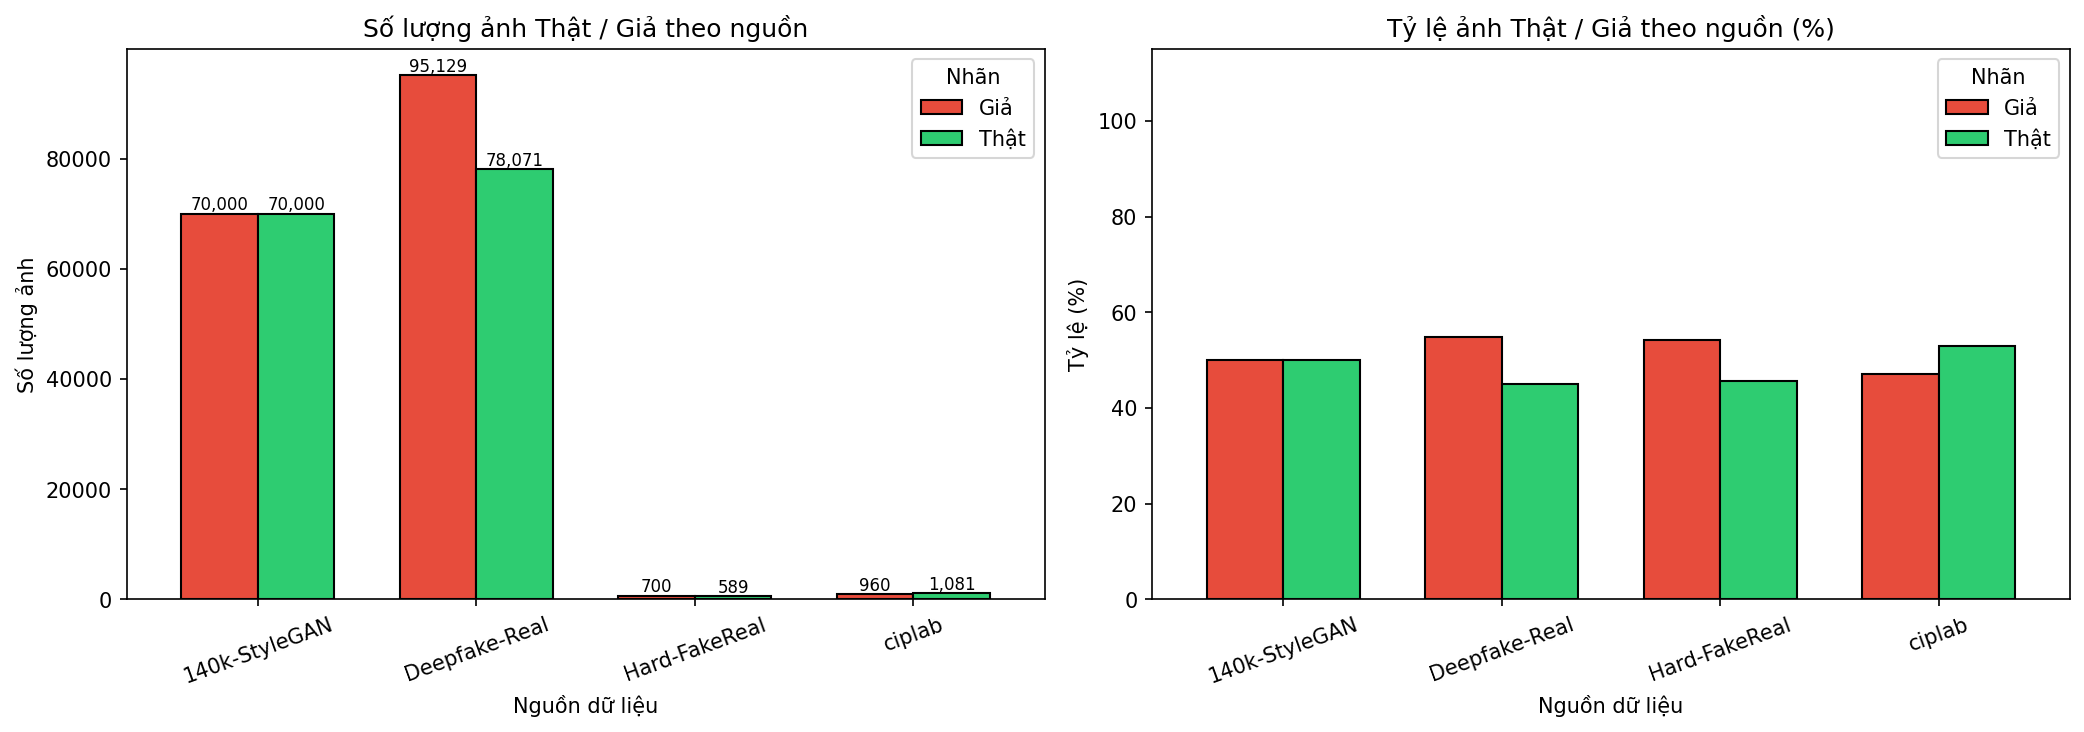
\includegraphics[width=0.85\linewidth]{eda/assets/eda_class_distribution.png}
  \caption{Phân bố số lượng ảnh thật và giả theo từng nguồn dữ liệu}
  \label{fig:class_dist}
\end{figure}

Bộ 140k-StyleGAN có phân bố hoàn toàn cân bằng (70.000 thật --- 70.000 giả) và chiếm khoảng 44\% tổng thể. Ưu thế quy mô của bộ này yêu cầu lưu ý: nếu không có chiến lược lấy mẫu phù hợp, mô hình có nguy cơ chủ yếu học đặc trưng của ảnh StyleGAN2.

\begin{table}[H]
  \centering
  \caption{Phân bố dữ liệu theo nguồn}
  \label{tab:source_dist}
  \begin{tabular}{lrrrr}
    \toprule
    \textbf{Nguồn} & \textbf{Tổng} & \textbf{Thật} & \textbf{Giả} & \textbf{T/G Ratio} \\
    \midrule
    140k-StyleGAN & 140.000 & 70.000 & 70.000 & 1,000 \\
    Deepfake-Real & 105.447 & 29.959 & 75.488 & 0,397 \\
    Hard-FakeReal & 1.289   &    589 &    700 & 0,841 \\
    ciplab        & 2.041   &  1.081 &    960 & 1,126 \\
    \midrule
    \textbf{Tổng cộng} & \textbf{248.777} & \textbf{101.629} & \textbf{147.148} & \textbf{0,691} \\
    \bottomrule
  \end{tabular}
\end{table}

\subsection{Phân Bố Độ Phân Giải}

\begin{figure}[H]
  \centering
  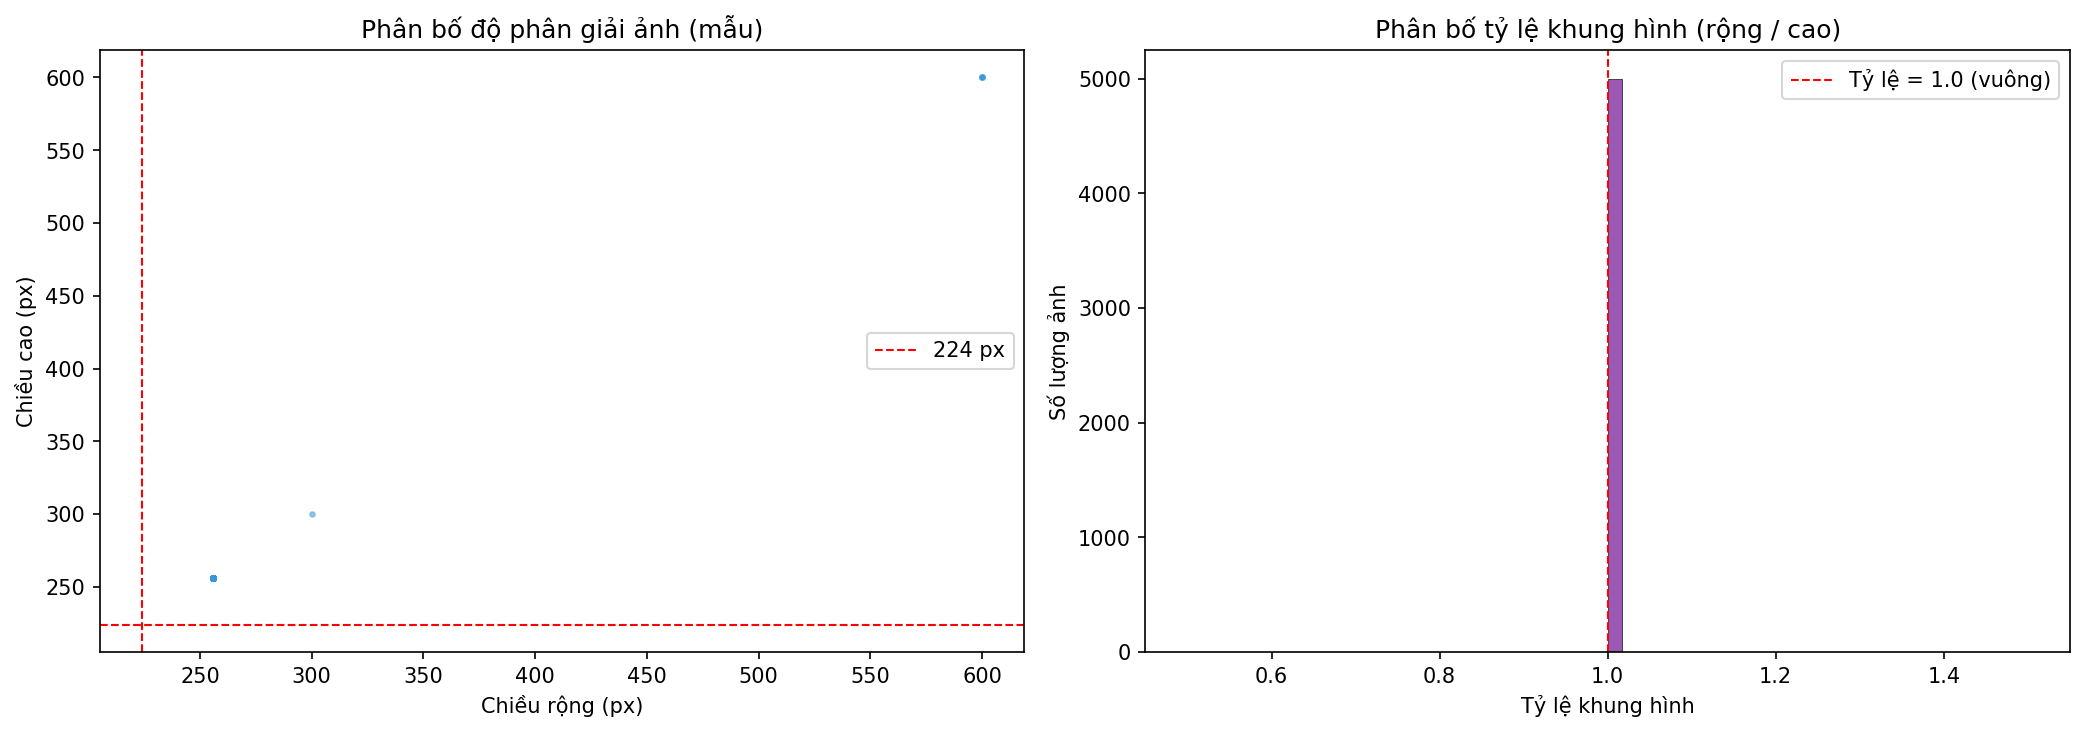
\includegraphics[width=0.85\linewidth]{eda/assets/eda_resolution.png}
  \caption{Phân bố độ phân giải và tỷ lệ khung hình của tập dữ liệu}
  \label{fig:resolution}
\end{figure}

Ảnh 140k-StyleGAN đã ở kích thước $224 \times 224$ --- phù hợp trực tiếp với EfficientNet-B0. Ảnh Deepfake-Real có kích thước gốc $256 \times 256$; resize về $224 \times 224$ chỉ mất tối thiểu thông tin. Hầu hết ảnh có tỷ lệ khung hình $\approx 1{:}1$ (vuông) --- resize không gây biến dạng hình học đáng kể.

\subsection{Phân Tích Thuộc Tính Pixel}

\begin{figure}[H]
  \centering
  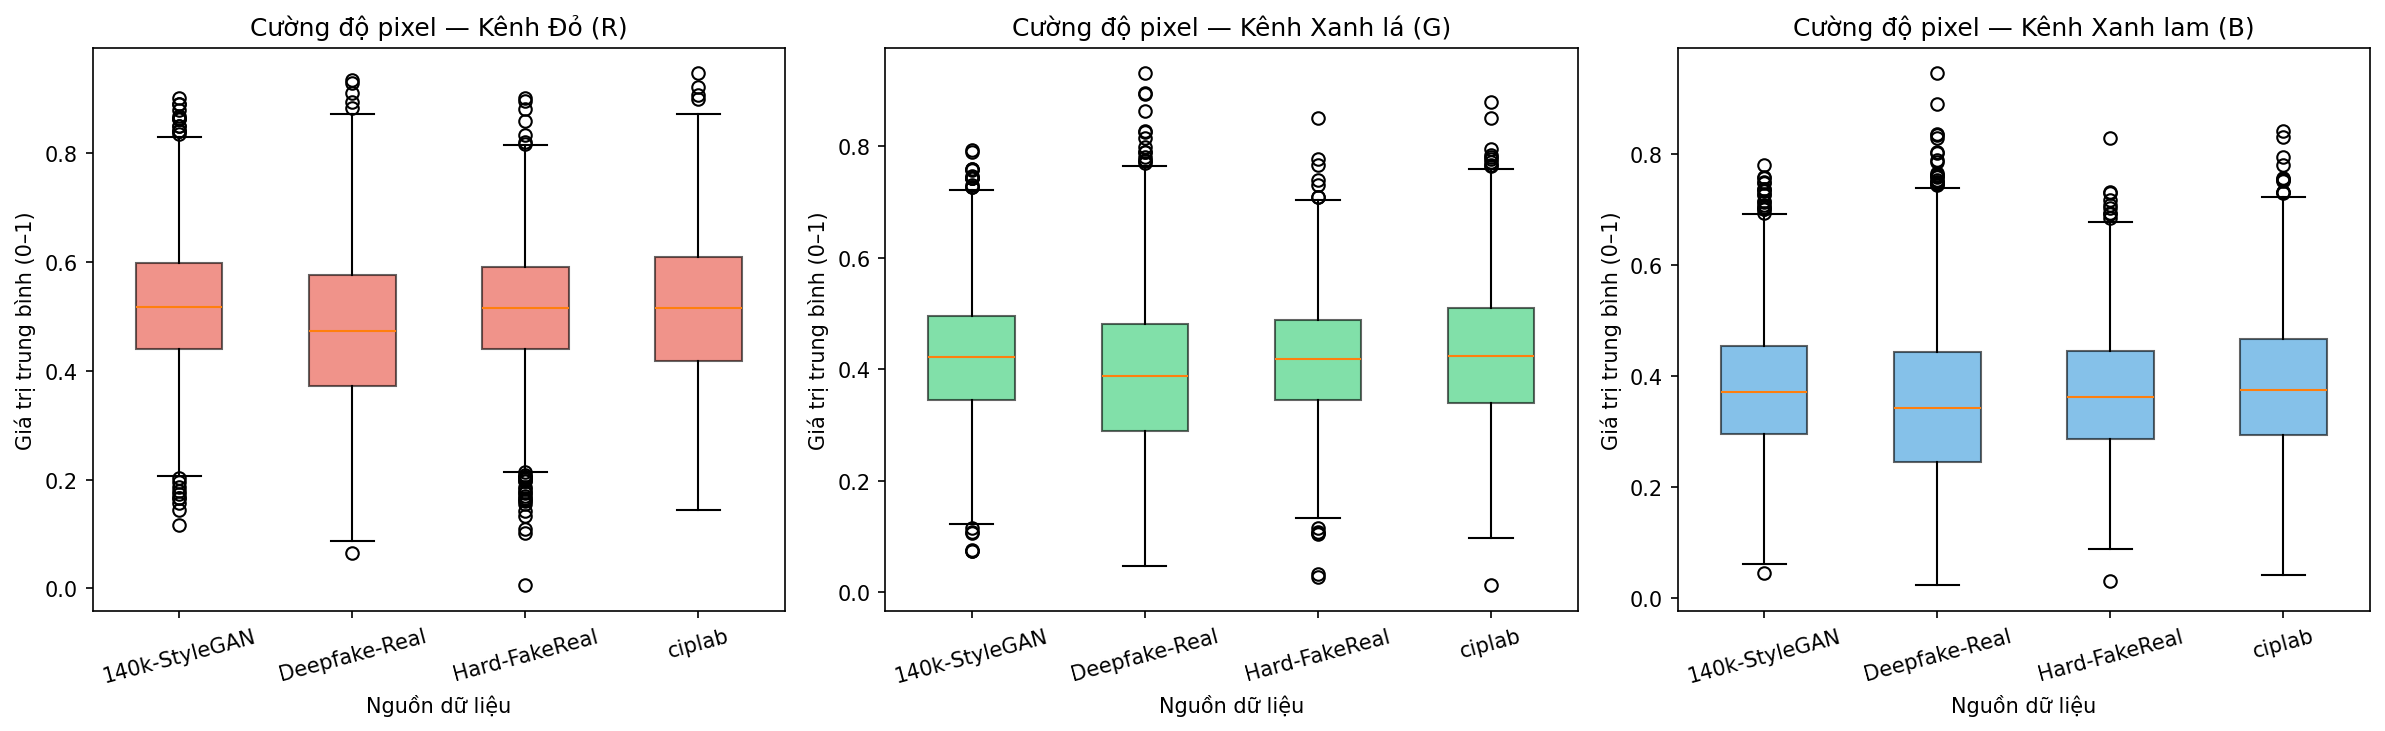
\includegraphics[width=0.85\linewidth]{eda/assets/eda_pixel_stats.png}
  \caption{Thống kê cường độ pixel R/G/B theo nguồn dữ liệu}
  \label{fig:pixel_stats}
\end{figure}

Phân bố pixel tương đối đồng nhất giữa bốn nguồn dữ liệu trong cùng kênh màu --- không có domain shift màu sắc cực đoan. Kênh R có xu hướng cao hơn kênh B, phù hợp với tông da người. Điều này xác nhận rằng chuẩn hóa ImageNet là lựa chọn phù hợp và không cần xử lý màu bổ sung.

\subsection{Phân Tích Mẫu Đại Diện}

\begin{figure}[H]
  \centering
  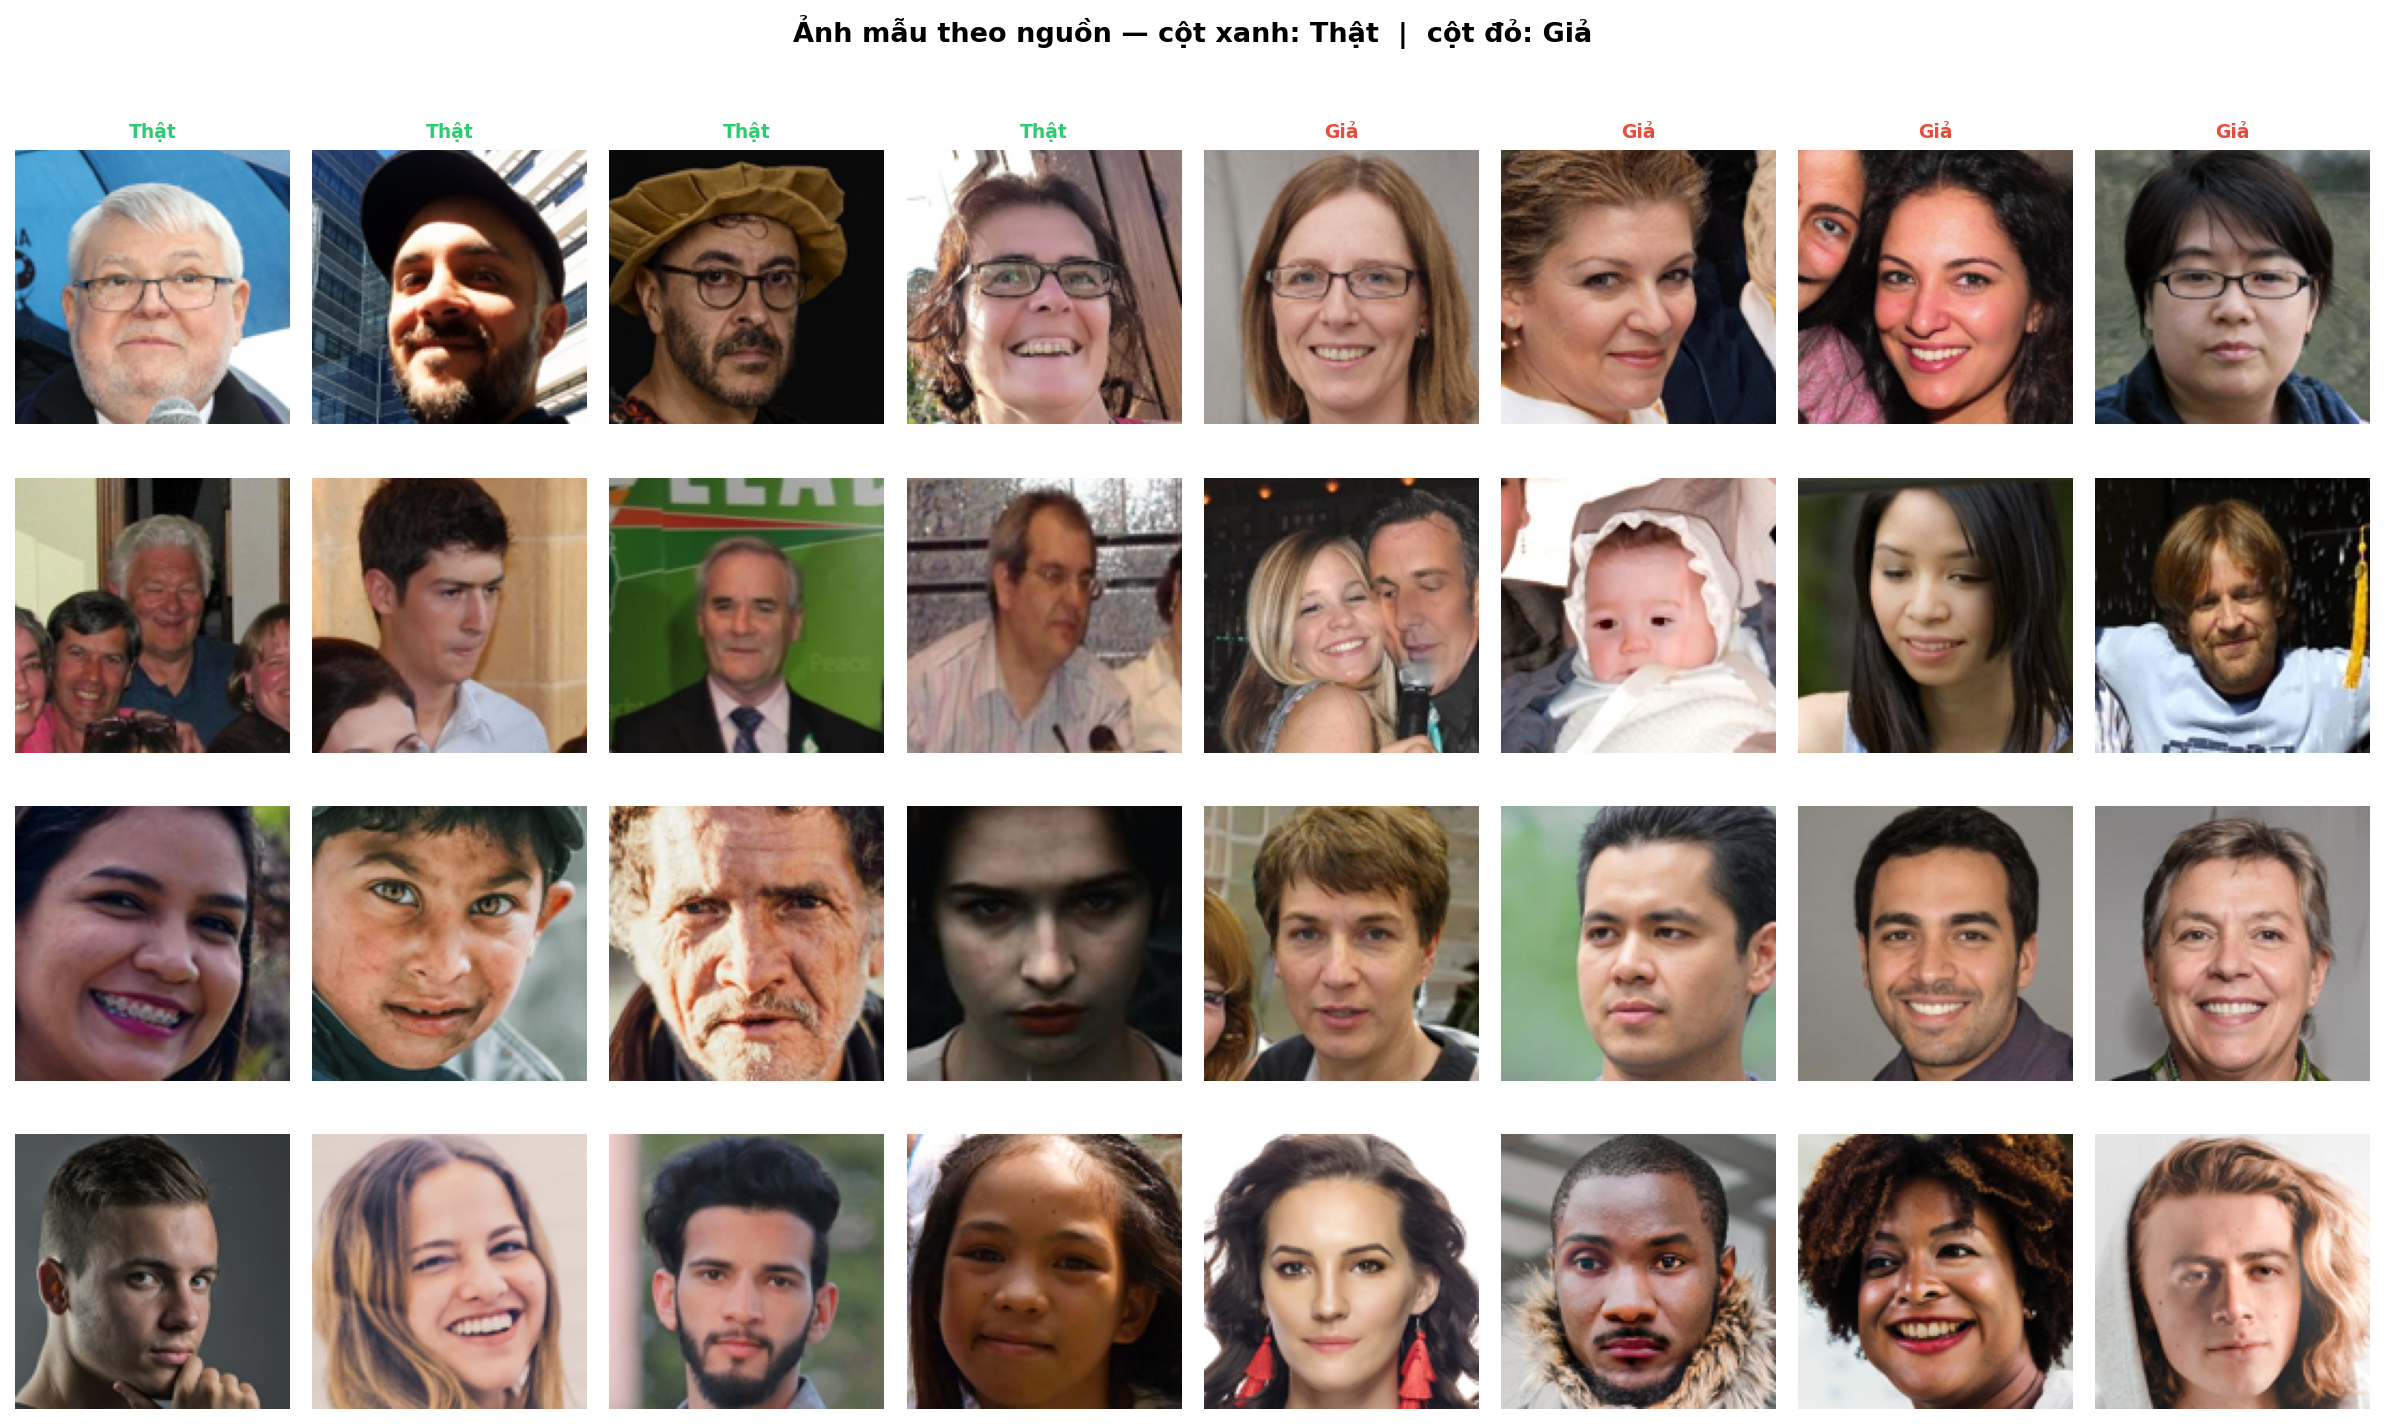
\includegraphics[width=\linewidth]{eda/assets/eda_sample_grid.png}
  \caption{Lưới ảnh mẫu: ảnh thật (viền xanh lá) và ảnh giả (viền đỏ) theo từng nguồn}
  \label{fig:sample_grid}
\end{figure}

Quan sát trực quan cho thấy sự khác biệt rõ rệt về đặc điểm artifact giữa các nguồn: StyleGAN2 để lại artifact ở vùng tai và tóc; deepfake manipulation-based có vùng biên khuôn mặt không tự nhiên; Hard-FakeReal được thiết kế để tối đa hóa độ khó phân biệt.

\subsection{Phân Tích Phổ Tần Số (FFT)}

\begin{figure}[H]
  \centering
  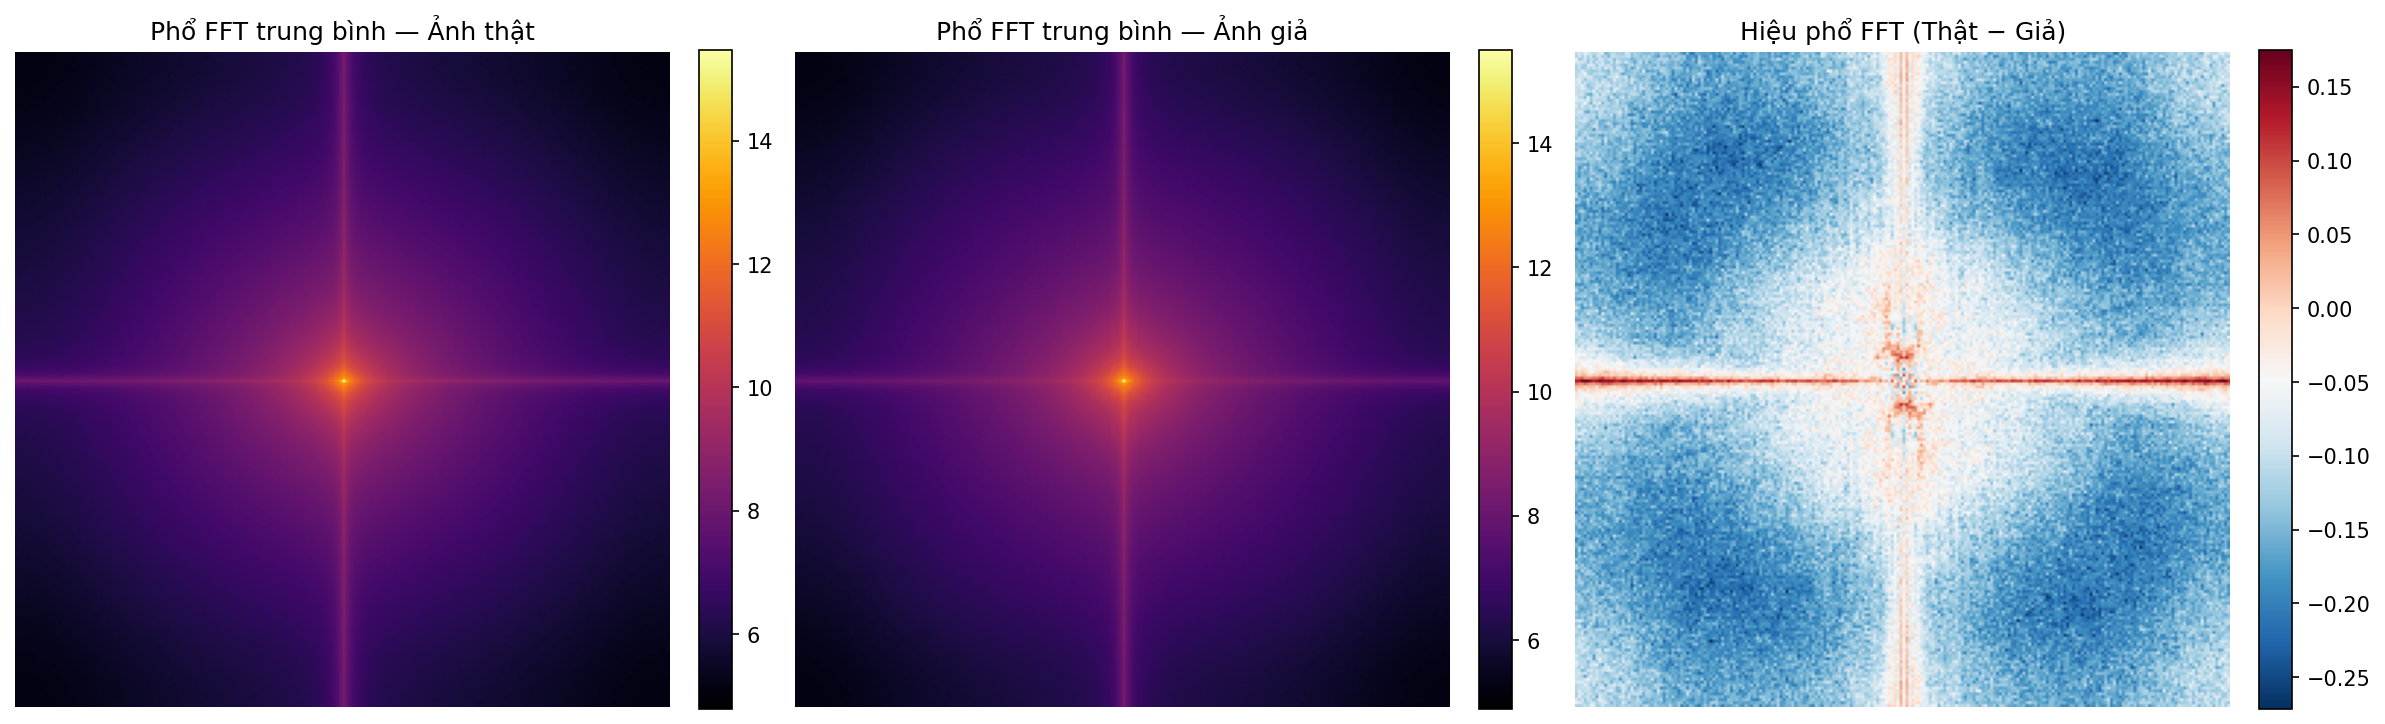
\includegraphics[width=0.85\linewidth]{eda/assets/eda_fft.png}
  \caption{Phân tích phổ FFT: phổ trung bình của ảnh thật (trái), ảnh giả (giữa) và hiệu phổ (phải)}
  \label{fig:fft}
\end{figure}

Phân tích FFT tiết lộ đặc điểm quan trọng: ảnh giả có năng lượng dư thừa ở mức chi tiết nhỏ (tần số cao) --- dấu vết của quá trình AI tạo ảnh. Hiệu phổ (Thật $-$ Giả) cho thấy ảnh giả thiếu sự mịn màng tự nhiên ở mức chi tiết vừa. Đây là cơ sở lý giải tại sao EfficientNet-B0 --- kiến trúc CNN học đặc trưng cục bộ ở nhiều mức độ --- là lựa chọn phù hợp.

\subsection{Kiểm Tra Tính Toàn Vẹn Dữ Liệu}

Kiểm tra chồng lấp giữa ba tập train/val/test bằng phép giao tập hợp đường dẫn ảnh xác nhận:
\begin{itemize}
  \item Train $\cap$ Val: $\emptyset$ (không trùng lặp)
  \item Train $\cap$ Test: $\emptyset$ (không trùng lặp)
  \item Val $\cap$ Test: $\emptyset$ (không trùng lặp)
\end{itemize}
Ba tập hoàn toàn độc lập --- kết quả đánh giá trên tập test là đáng tin cậy và không bị ảnh hưởng bởi rò rỉ dữ liệu.

\section{Nhận Xét Chất Lượng Bộ Dữ Liệu}

\subsection{Kích Thước và Cấu Trúc}

Với tổng cộng \textbf{316.530 ảnh} sau loại bỏ trùng lặp MD5 --- trong đó 221.571 ảnh dùng để huấn luyện --- bộ dữ liệu có quy mô đủ lớn để huấn luyện mô hình deep learning. Mức độ mất cân bằng lớp nhẹ (47,3\% thật --- 52,7\% giả) không đòi hỏi điều chỉnh trọng số lớp: Precision cao (97,73\%) trên tập test bác bỏ giả thuyết mô hình thiên vị về lớp đa số.

\subsection{Thách Thức Kỹ Thuật}

\begin{itemize}
  \item \textbf{Domain shift giữa các nguồn:} Bốn bộ dữ liệu khác nhau về phương pháp sinh ảnh, độ phân giải gốc và đặc điểm artifact. Đây là lý do cốt lõi để thiết kế bài kiểm tra cross-generator.

  \item \textbf{Hard-FakeReal:} Bộ dữ liệu này đặc biệt thách thức do ảnh giả được thiết kế có chủ đích để khó phân biệt --- mô hình cần học đặc trưng tinh vi ở mức pixel.

  \item \textbf{Ưu thế số lượng của 140k-StyleGAN ($\approx 44\%$):} Cần đảm bảo mô hình không học thiên về phong cách ảnh StyleGAN2 mà bỏ qua đặc trưng của các bộ còn lại.
\end{itemize}

\chapter{PHƯƠNG PHÁP ĐỀ XUẤT}

\section{Mô Hình}

\subsection{EfficientNet-B0 Backbone}

Kiến trúc backbone được chọn là EfficientNet-B0 \cite{tan2019efficientnet}, nạp từ thư viện timm \cite{wightman2019timm} với trọng số tiền huấn luyện trên ImageNet:

\begin{lstlisting}[style=python, caption={Khởi tạo EfficientNet-B0 backbone}]
import timm
backbone = timm.create_model(
    "efficientnet_b0",
    pretrained=True,
    num_classes=0,   # loai bo classifier mac dinh
    global_pool=""   # them pooling rieng
)
# output: feature map (B, 1280, 7, 7)
\end{lstlisting}

EfficientNet được xây dựng trên nguyên tắc \textit{compound scaling} --- scale đồng thời độ sâu (depth), độ rộng (width) và độ phân giải (resolution) theo một hệ số tỷ lệ thống nhất. EfficientNet-B0 --- phiên bản nhỏ nhất --- đạt accuracy tương đương ResNet-50 với $\approx 5{,}3$M tham số (so với $\approx 25{,}6$M), phù hợp fine-tuning trên tập dữ liệu đa domain.

\begin{table}[H]
  \centering
  \caption{So sánh kiến trúc backbone}
  \label{tab:backbone_compare}
  \begin{tabular}{llrl}
    \toprule
    \textbf{Kiến trúc} & \textbf{Tham số} & \textbf{Top-1 Acc. (ImageNet)} & \textbf{Ghi chú} \\
    \midrule
    EfficientNet-B0 & $\approx$5,3M & 77,1\% & \textit{Lựa chọn đề tài} \\
    ResNet-50       & $\approx$25,6M & 76,2\% & $\approx 5\times$ tham số hơn \\
    VGG-16          & $\approx$138M  & 74,4\% & Quá nặng cho fine-tuning \\
    ViT-B/16        & $\approx$86M   & 81,8\% & Cần nhiều dữ liệu hơn \\
    \bottomrule
  \end{tabular}
\end{table}

\subsection{Custom Classification Head}

Sau backbone, một phần đầu phân loại tùy chỉnh được gắn vào:

\begin{figure}[H]
  \centering
  \begin{minipage}{0.55\linewidth}
    \begin{lstlisting}[style=python, caption={Kiến trúc classification head}]
nn.Sequential(
    nn.AdaptiveAvgPool2d(1),  # (B,1280,1,1)
    nn.Flatten(),              # (B, 1280)
    nn.Linear(1280, 256),
    nn.ReLU(inplace=True),
    nn.Dropout(p=0.5),
    nn.Linear(256, 1)          # logit
)
    \end{lstlisting}
  \end{minipage}
\end{figure}

\begin{table}[H]
  \centering
  \caption{Thiết kế và lý do từng thành phần trong classification head}
  \label{tab:head}
  \begin{tabularx}{\linewidth}{llX}
    \toprule
    \textbf{Thành phần} & \textbf{Cấu hình} & \textbf{Lý do thiết kế} \\
    \midrule
    AdaptiveAvgPool2d & Output (1,1) & Tổng hợp không gian từ toàn bộ feature map \\
    Linear (đầu tiên) & $1280 \to 256$ & Đủ rộng để học ranh giới phân loại Real/Fake \\
    Dropout           & $p = 0{,}5$   & Ngăn overfitting --- artifact dễ bị ``học thuộc'' \\
    Linear (đầu ra)   & $256 \to 1$   & Một logit cho phân loại nhị phân \\
    \bottomrule
  \end{tabularx}
\end{table}

\textbf{Hàm mất mát:} \texttt{BCEWithLogitsLoss} kết hợp sigmoid và binary cross-entropy:
\begin{equation}
  \mathcal{L}(x, y) = -\bigl[ y \cdot \log\sigma(x) + (1-y) \cdot \log(1 - \sigma(x)) \bigr]
  \label{eq:bce}
\end{equation}
trong đó $x$ là logit đầu ra, $y \in \{0, 1\}$ là nhãn thật, $\sigma(\cdot)$ là hàm sigmoid. Sigmoid \textbf{không} được áp dụng trước khi tính mất mát --- chỉ áp dụng khi inference.

\subsection{Sơ Đồ Kiến Trúc Tổng Thể}

Hình~\ref{fig:model_architecture} trực quan hóa luồng dữ liệu qua toàn bộ mô hình từ ảnh đầu vào đến quyết định phân loại cuối cùng.

\begin{figure}[H]
  \centering
  \begin{tikzpicture}[
    node distance=0.52cm,
    every node/.style={font=\small},
    bk/.style  = {rectangle, draw=orange!70!black, fill=orange!7, rounded corners=3pt,
                  minimum width=9.5cm, minimum height=0.88cm, align=center},
    hd/.style  = {rectangle, draw=green!60!black, fill=green!7, rounded corners=3pt,
                  minimum width=9.5cm, minimum height=0.88cm, align=center},
    io/.style  = {rectangle, draw=uitblue, fill=uitblue!8, rounded corners=3pt,
                  minimum width=9.5cm, minimum height=0.88cm, align=center},
    arr/.style = {-Stealth, semithick}
  ]
    \node[io] (inp)  {Ảnh đầu vào $\;\big|\;$ Resize($224{\times}224$) $\;\big|\;$ Normalize (ImageNet)};
    \node[bk, below=of inp]  (bk0)
      {EfficientNet-B0: MBConv Blocks 0--4 \quad \textit{(đóng băng ở Giai đoạn 1--2)}};
    \node[bk, below=of bk0]  (bk1)
      {EfficientNet-B0: MBConv Blocks 5--6 \quad \textit{(mở băng từ Giai đoạn 2)}};
    \node[bk, below=of bk1]  (fm)
      {Feature Map $\quad 1280 \times 7 \times 7$};
    \node[hd, below=of fm]   (gp)
      {AdaptiveAvgPool2d(1,1) $\;\to\;$ Flatten $\;\to\;$ $\mathbb{R}^{1280}$};
    \node[hd, below=of gp]   (fc1)
      {Linear(1280, 256) $\;\to\;$ ReLU $\;\to\;$ Dropout(0.5)};
    \node[hd, below=of fc1]  (fc2)
      {Linear(256, 1) \quad Logit $\in \mathbb{R}$};
    \node[io, below=of fc2]  (out)
      {Sigmoid $\to$ $p \in [0,1]$ $\;\;\big|\;\;$ Real ($p \leq 0{,}5$) $\;/\;$ Fake ($p > 0{,}5$)};

    \foreach \a/\b in {inp/bk0, bk0/bk1, bk1/fm, fm/gp, gp/fc1, fc1/fc2, fc2/out}
      \draw[arr] (\a.south) -- (\b.north);
  \end{tikzpicture}
  \caption{Kiến trúc tổng thể mô hình EfficientNet-B0 với classification head tùy chỉnh.
           Cam: EfficientNet-B0 backbone pretrained. Xanh lá: custom classification head.}
  \label{fig:model_architecture}
\end{figure}

\subsection{Chiến Lược Huấn Luyện 3 Giai Đoạn}

Chiến lược dựa trên nguyên tắc \textit{discriminative fine-tuning}: các lớp gần đầu vào đã học đặc trưng tốt từ ImageNet nên cần learning rate thấp; các lớp đầu ra mới cần học từ đầu với learning rate cao hơn.

\begin{table}[H]
  \centering
  \caption{Thông số chi tiết 3 giai đoạn huấn luyện}
  \label{tab:stages}
  \begin{tabularx}{\linewidth}{clXrrl}
    \toprule
    \textbf{GĐ} & \textbf{Tên} & \textbf{Lớp trainable} & \textbf{LR} & \textbf{Max E.} & \textbf{Checkpoint} \\
    \midrule
    1 & Freeze Backbone   & Head only                   & $10^{-4}$ & 30 & \texttt{best\_stage1.pth} \\
    2 & Unfreeze Top      & Head + blocks 5--6          & $10^{-5}$ & 30 & \texttt{best\_stage2.pth} \\
    3 & Unfreeze All      & Toàn bộ mô hình             & $10^{-6}$ & 30 & \texttt{best\_stage3.pth} \\
    \bottomrule
  \end{tabularx}
\end{table}

\begin{table}[H]
  \centering
  \caption{Kết quả huấn luyện trên tập kiểm định theo giai đoạn}
  \label{tab:train_results}
  \begin{tabular}{clrrrl}
    \toprule
    \textbf{GĐ} & \textbf{Epochs chạy} & \textbf{Val Loss} & \textbf{Val Accuracy} & \textbf{Kích thước} \\
    \midrule
    1 & 30/30 & 0,3103 & 86,63\% & 20,3 MB \\
    2 & 30/30 & 0,1383 & 94,54\% & 26,0 MB \\
    3 & 30/30 & 0,0699 & 97,34\% & 52,5 MB \\
    \bottomrule
  \end{tabular}
\end{table}

Đáng chú ý, EarlyStopping không kích hoạt ở bất kỳ giai đoạn nào --- mô hình tiếp tục cải thiện đến epoch cuối. Val loss giảm liên tục $0{,}310 \to 0{,}138 \to 0{,}070$ ($\approx 77\%$ tổng mức giảm).

Hình~\ref{fig:training_stages} trình bày sơ đồ luồng toàn bộ quy trình huấn luyện 3 giai đoạn, từ khởi tạo mô hình đến đánh giá trên tập test độc lập.

\begin{figure}[H]
  \centering
  \begin{tikzpicture}[
    every node/.style={font=\small},
    stage/.style = {rectangle, draw=uitblue, fill=uitblue!10, rounded corners=4pt,
                    minimum width=3.4cm, minimum height=2.6cm, align=center},
    res/.style   = {rectangle, draw=green!60!black, fill=green!7, rounded corners=3pt,
                    text width=3.2cm, minimum height=0.88cm, align=center, font=\footnotesize},
    fin/.style   = {rectangle, draw=orange!70!black, fill=orange!8, rounded corners=4pt,
                    minimum width=11.5cm, minimum height=0.95cm, align=center},
    arr/.style   = {-Stealth, semithick, uitblue}
  ]
    \node[stage] (s1) at (0,0) {
      \textbf{Giai đoạn 1}\\[4pt]
      \small Freeze Backbone\\
      LR $= 10^{-4}$\\
      30 epochs\\
      Head only
    };
    \node[stage] (s2) at (4.2,0) {
      \textbf{Giai đoạn 2}\\[4pt]
      \small Unfreeze B5--B6\\
      LR $= 10^{-5}$\\
      30 epochs\\
      Head + Blocks 5--6
    };
    \node[stage] (s3) at (8.4,0) {
      \textbf{Giai đoạn 3}\\[4pt]
      \small Full Fine-tune\\
      LR $= 10^{-6}$\\
      30 epochs\\
      Toàn bộ mô hình
    };

    \node[res, below=0.5cm of s1] (r1) {Val Acc: 86,63\%\\Val Loss: 0,310};
    \node[res, below=0.5cm of s2] (r2) {Val Acc: 94,54\%\\Val Loss: 0,138};
    \node[res, below=0.5cm of s3] (r3) {Val Acc: 97,34\%\\Val Loss: 0,070};

    % eval positioned directly below middle result — no empty space
    \node[fin, below=0.75cm of r2] (eval) {
      Đánh giá trên Test Set (47.480 ảnh):
      \quad Acc 97,33\% $\;|\;$ F1 97,45\% $\;|\;$ AUC-ROC 99,70\%
    };

    % Horizontal arrows — label slightly raised to clear box border
    \draw[arr] (s1.east) -- node[above, font=\footnotesize\itshape, yshift=1pt] {checkpoint} (s2.west);
    \draw[arr] (s2.east) -- node[above, font=\footnotesize\itshape, yshift=1pt] {checkpoint} (s3.west);

    % Vertical arrows from stages to results
    \foreach \s/\r in {s1/r1, s2/r2, s3/r3}
      \draw[-Stealth, semithick] (\s.south) -- (\r.north);

    % Three vertical arrows converging straight down into eval.north
    \draw[-Stealth, semithick] (r1.south) -- (r1.south |- eval.north);
    \draw[-Stealth, semithick] (r2.south) -- (eval.north);
    \draw[-Stealth, semithick] (r3.south) -- (r3.south |- eval.north);
  \end{tikzpicture}
  \caption{Sơ đồ chiến lược huấn luyện 3 giai đoạn progressive unfreezing và kết quả từng giai đoạn}
  \label{fig:training_stages}
\end{figure}

\section{Pipeline Tiền Xử Lý và Tăng Cường Dữ Liệu}

\subsection{Tiền Xử Lý Cơ Bản}

Mọi ảnh đầu vào trải qua hai bước cố định:
\begin{enumerate}
  \item \textbf{Resize về $224 \times 224$:} Kích thước đầu vào mặc định của EfficientNet-B0. EDA xác nhận hầu hết ảnh đã ở tỷ lệ khung hình $\approx 1{:}1$, không gây biến dạng.
  \item \textbf{Chuẩn hóa ImageNet:} Mean $= [0{,}485;\ 0{,}456;\ 0{,}406]$, Std $= [0{,}229;\ 0{,}224;\ 0{,}225]$ (kênh R/G/B).
\end{enumerate}

\subsection{Tăng Cường Dữ Liệu (Train Only)}

\begin{table}[H]
  \centering
  \caption{Các phép biến đổi tăng cường dữ liệu (albumentations)}
  \label{tab:augmentation}
  \begin{tabularx}{\linewidth}{lXrl}
    \toprule
    \textbf{Phép biến đổi} & \textbf{Tham số} & \textbf{$p$} & \textbf{Mục đích} \\
    \midrule
    HorizontalFlip & --- & 0,5 & Mô phỏng đối xứng gương \\
    RandomBrightnessContrast & brightness\_limit=0,2; contrast\_limit=0,2 & 0,5 & Mô phỏng điều kiện ánh sáng \\
    ShiftScaleRotate & shift=0,1; scale=0,1; rotate=15° & 0,5 & Mô phỏng góc chụp thay đổi \\
    CoarseDropout & max\_holes=8; kích thước $16{\times}16$~px & 0,3 & Ngăn phụ thuộc đặc trưng cục bộ \\
    \bottomrule
  \end{tabularx}
\end{table}

Tập val/test chỉ áp dụng resize và chuẩn hóa --- không augmentation để đảm bảo đánh giá tái lập.

\section{Môi Trường Huấn Luyện và Công Nghệ Sử Dụng}

Mô hình được huấn luyện trong $\approx 17$ giờ trên phần cứng dưới đây.

\begin{table}[H]
  \centering
  \caption{Cấu hình phần cứng huấn luyện}
  \label{tab:hardware}
  \begin{tabular}{ll}
    \toprule
    \textbf{Thành phần} & \textbf{Thông số} \\
    \midrule
    CPU  & AMD Ryzen 5 7500F 6-Core \\
    GPU  & NVIDIA GeForce RTX 5070 \\
    VRAM & 12,82 GB \\
    Compute Capability & 12.0 (Blackwell) \\
    CUDA & 13.0 \\
    \bottomrule
  \end{tabular}
\end{table}

\begin{table}[H]
  \centering
  \caption{Các thư viện và phiên bản sử dụng}
  \label{tab:libraries}
  \begin{tabular}{llll}
    \toprule
    \textbf{Loại} & \textbf{Thư viện} & \textbf{Phiên bản} & \textbf{Mục đích} \\
    \midrule
    Framework     & PyTorch       & 2.12.0+cu130 & Deep learning \\
    Model library & timm          & 1.0.27       & EfficientNet-B0 pretrained \\
    Augmentation  & albumentations & 2.0.8       & Train transform \\
    Metrics       & scikit-learn  & 1.8.0        & Acc/P/R/F1/AUC-ROC \\
    Visualization & matplotlib    & $\geq$3.8    & Confusion matrix, ROC curve \\
    Data          & pandas        & $\geq$2.1    & Đọc và xử lý CSV \\
    Config        & PyYAML        & ---          & Nạp siêu tham số từ YAML \\
    Ngôn ngữ      & Python        & 3.12         & --- \\
    \bottomrule
  \end{tabular}
\end{table}

\textbf{Mixed-precision training (FP16):} Được bật bằng \texttt{torch.cuda.amp.autocast()} kết hợp \texttt{GradScaler}, giảm VRAM $\approx 40\%$ và tăng tốc $\approx 1{,}5$--$2\times$ trên RTX 5070.

\textbf{Tái lập kết quả:} Seed 42 cố định cho \texttt{random}, \texttt{numpy}, \texttt{torch} và \texttt{torch.cuda}; \texttt{deterministic=True}.

\section{Lớp FaceDataset và DataLoader}

\subsection{Thiết Kế Lớp FaceDataset}

Lớp \texttt{FaceDataset} (định nghĩa tại \texttt{src/dataset.py}) kế thừa \texttt{torch.utils.data.Dataset} và đóng vai trò giao diện giữa file CSV phân chia và pipeline huấn luyện. Luồng xử lý bên trong \texttt{\_\_getitem\_\_} gồm ba bước:

\begin{enumerate}
  \item Đọc đường dẫn ảnh và nhãn từ DataFrame đã nạp trong \texttt{\_\_init\_\_}.
  \item Mở ảnh bằng \texttt{PIL.Image.open()}, chuyển sang mảng NumPy RGB, áp dụng transform (albumentations hoặc chỉ resize+normalize cho val/test).
  \item Trả về cặp \texttt{(image\_tensor, label\_tensor)} với \texttt{label\_tensor} kiểu \texttt{torch.float32} --- kiểu dữ liệu bắt buộc bởi \texttt{BCEWithLogitsLoss}.
\end{enumerate}

\subsection{Cấu Hình DataLoader}

\begin{table}[H]
  \centering
  \caption{Cấu hình DataLoader cho ba tập dữ liệu}
  \label{tab:dataloader}
  \begin{tabular}{llll}
    \toprule
    \textbf{Tham số} & \textbf{Train} & \textbf{Val} & \textbf{Test} \\
    \midrule
    batch\_size   & 128  & 128  & 128  \\
    shuffle       & True & False & False \\
    num\_workers  & 2    & 2    & 2    \\
    pin\_memory   & True & True & True \\
    drop\_last    & False & False & False \\
    \bottomrule
  \end{tabular}
\end{table}

\textbf{Lý do chọn \texttt{num\_workers=2}:} Trên hệ thống với CPU 6 nhân, \texttt{num\_workers=4} gây tranh chấp tài nguyên với tiến trình huấn luyện chính. Qua thử nghiệm, giá trị 2 cho thời gian nạp dữ liệu đủ nhanh để GPU không bị đợi (bottleneck tại data loading $<$ 5\% thời gian mỗi batch).

\subsection{Quy Trình Quản Lý Siêu Tham Số}

Toàn bộ siêu tham số được khai báo tập trung trong \texttt{configs/train\_config.yaml}. Không có giá trị nào được hardcode trong mã nguồn. Khi khởi chạy, script đọc file YAML, ghi log đầy đủ các tham số cùng với phiên bản thư viện và thông tin GPU, đảm bảo mọi lần chạy đều có thể tái lập và truy xuất cấu hình sau này.

Quy trình quản lý thực nghiệm này --- seed cố định, tham số qua YAML, log phiên bản --- là thực hành tốt trong nghiên cứu học sâu để đảm bảo tính tái lập (reproducibility), một yêu cầu ngày càng được nhấn mạnh trong cộng đồng ML nghiên cứu.

\chapter{THỰC NGHIỆM}

\section{Quy Trình Thực Nghiệm}

\subsection{Xử Lý Dữ Liệu}

Quy trình chuẩn bị dữ liệu thực hiện qua hai notebook tuần tự:
\begin{itemize}
  \item \textbf{\texttt{00\_download\_datasets.ipynb}:} Tải bốn bộ Kaggle về \texttt{data/raw/}. Idempotent --- bỏ qua các bộ đã tồn tại.
  \item \textbf{\texttt{01\_dataset\_preparation.ipynb}:} MD5 dedup $\to$ class balance check $\to$ EDA plots $\to$ stratified split 70/15/15 $\to$ xuất CSV.
\end{itemize}

Kết quả: \textbf{316.530 ảnh} (221.571 train / 47.479 val / 47.480 test), phân bố nhãn đồng đều 47,3\% thật --- 52,7\% giả trên cả ba tập.

\subsection{Chuẩn Bị Dữ Liệu Cho Mô Hình}

\begin{itemize}
  \item \textbf{Tập train:} resize $224{\times}224$ $\to$ augmentation $\to$ chuẩn hóa ImageNet $\to$ \texttt{torch.Tensor}.
  \item \textbf{Tập val/test:} resize $224{\times}224$ $\to$ chuẩn hóa ImageNet (không augmentation).
  \item \textbf{DataLoader:} batch\_size=128, num\_workers=2, pin\_memory=True.
\end{itemize}

Seed tái lập cố định ở mức 42. Phiên bản ghi nhận khi bắt đầu chạy: PyTorch 2.12.0+cu130, timm 1.0.27, GPU NVIDIA GeForce RTX 5070.

\section{Độ Đo Đánh Giá}

Kết quả cuối cùng được báo cáo chỉ trên tập kiểm tra (47.480 ảnh), tính bằng \texttt{sklearn.metrics}.

\begin{table}[H]
  \centering
  \caption{Định nghĩa và ý nghĩa các độ đo đánh giá}
  \label{tab:metrics_def}
  \begin{tabularx}{\linewidth}{llX}
    \toprule
    \textbf{Độ đo} & \textbf{Công thức} & \textbf{Ý nghĩa trong bài toán} \\
    \midrule
    Accuracy  & $\frac{TP+TN}{TP+TN+FP+FN}$ & Tỷ lệ ảnh phân loại đúng tổng thể \\
    Precision & $\frac{TP}{TP+FP}$ & Trong số ảnh dự đoán là giả, bao nhiêu thực sự là giả \\
    Recall    & $\frac{TP}{TP+FN}$ & Trong số ảnh giả thực tế, bao nhiêu được phát hiện đúng \\
    F1-Score  & $\frac{2 \cdot P \cdot R}{P + R}$ & Trung bình điều hòa Precision và Recall \\
    AUC-ROC   & Diện tích dưới ROC & Khả năng phân biệt Real/Fake ở mọi ngưỡng threshold \\
    \bottomrule
  \end{tabularx}
\end{table}

Recall quan trọng hơn Precision vì bỏ sót ảnh giả (False Negative) gây hại thực tế nhiều hơn cảnh báo nhầm. AUC-ROC là độ đo tổng hợp tin cậy nhất vì không phụ thuộc vào ngưỡng phân loại cụ thể. \textit{Positive class} = Fake (1).

\section{Thông Số Chi Tiết Các Giai Đoạn Huấn Luyện}

\begin{table}[H]
  \centering
  \caption{Siêu tham số chung cho toàn bộ quá trình huấn luyện}
  \label{tab:hyperparam}
  \begin{tabular}{lll}
    \toprule
    \textbf{Tham số} & \textbf{Giá trị} & \textbf{Nguồn} \\
    \midrule
    Optimizer          & AdamW \cite{loshchilov2019adamw} & \texttt{train\_config.yaml} \\
    Weight decay       & $10^{-4}$                        & \texttt{train\_config.yaml} \\
    Batch size         & 128                              & \texttt{train\_config.yaml} \\
    Max epochs/stage   & 30                               & \texttt{train\_config.yaml} \\
    Mixed precision    & FP16 (autocast + GradScaler)     & \texttt{train\_config.yaml} \\
    EarlyStopping      & patience=5, monitor: val\_loss   & \texttt{train\_config.yaml} \\
    ReduceLROnPlateau  & patience=3, factor=0,3, min\_lr=$10^{-7}$ & \texttt{train\_config.yaml} \\
    Random seed        & 42                               & \texttt{train\_config.yaml} \\
    \bottomrule
  \end{tabular}
\end{table}

\section{Đánh Giá Thực Nghiệm}

\subsection{Kết Quả Trên Tập Kiểm Tra}

Đánh giá thực hiện trên tập kiểm tra độc lập (47.480 ảnh) với checkpoint tốt nhất của Giai đoạn 3 (\texttt{best\_stage3.pth}, val\_loss=$0{,}0699$).

\begin{table}[H]
  \centering
  \caption{Kết quả đánh giá trên tập kiểm tra --- checkpoint Stage 3}
  \label{tab:test_results}
  \begin{tabular}{lrr}
    \toprule
    \textbf{Độ đo} & \textbf{Giá trị} & \textbf{(\%)} \\
    \midrule
    Accuracy  & 0,9733 & 97,33\% \\
    Precision & 0,9773 & 97,73\% \\
    Recall    & 0,9718 & 97,18\% \\
    F1-Score  & 0,9745 & 97,45\% \\
    AUC-ROC   & 0,9970 & 99,70\% \\
    \bottomrule
  \end{tabular}
  \newline
  {\small Nguồn: \texttt{artifacts/results/metrics.txt}}
\end{table}

\begin{table}[H]
  \centering
  \caption{So sánh kết quả qua các giai đoạn trên tập kiểm định}
  \label{tab:stage_compare}
  \begin{tabular}{lccc}
    \toprule
    \textbf{Giai đoạn} & \textbf{Val Accuracy} & \textbf{Cải thiện} \\
    \midrule
    1 (Head only)       & 86,63\% & --- \\
    2 (Partial unfreeze) & 94,54\% & $+7{,}91$ pp \\
    3 (Full fine-tune)  & 97,34\% & $+2{,}80$ pp \\
    \bottomrule
  \end{tabular}
\end{table}

\begin{figure}[H]
  \centering
  \begin{subfigure}{0.48\linewidth}
    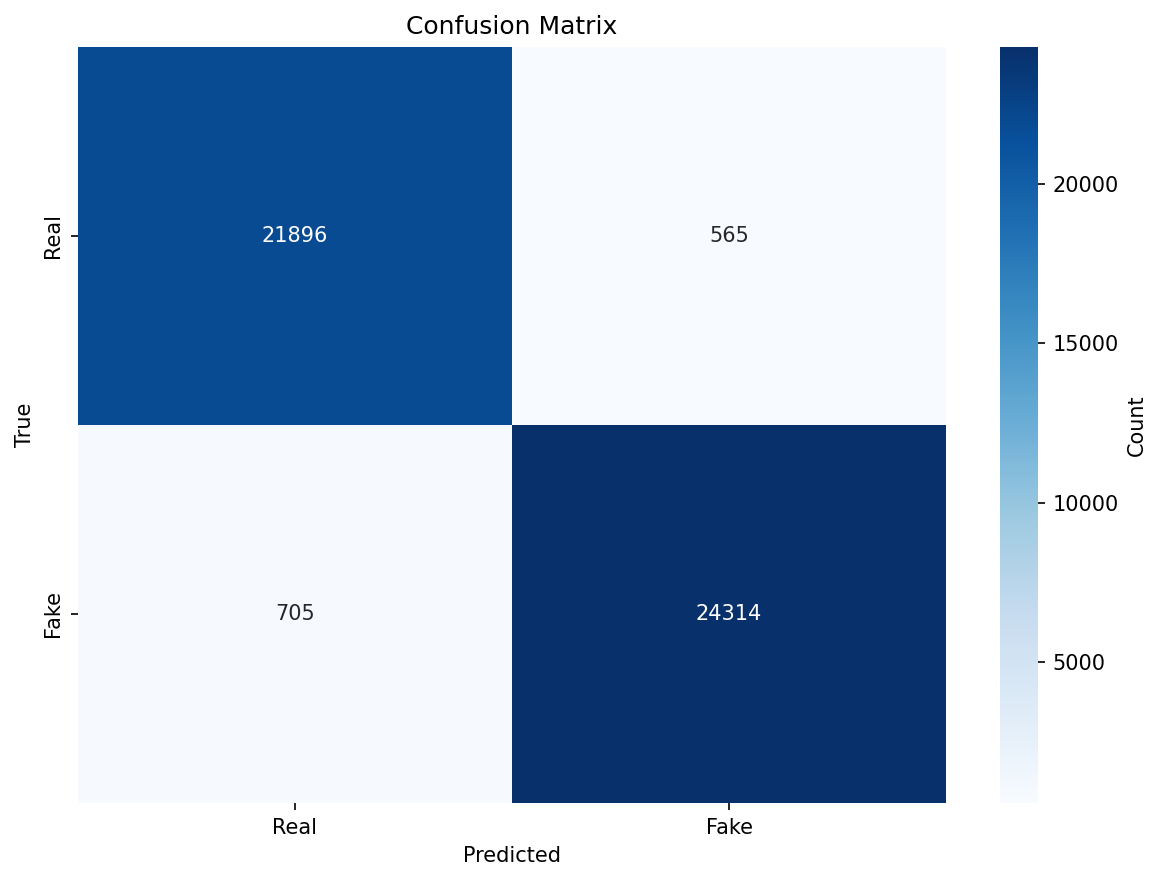
\includegraphics[width=\linewidth]{../../artifacts/results/confusion_matrix.png}
    \caption{Ma trận nhầm lẫn (tập test)}
    \label{fig:confusion}
  \end{subfigure}
  \hfill
  \begin{subfigure}{0.48\linewidth}
    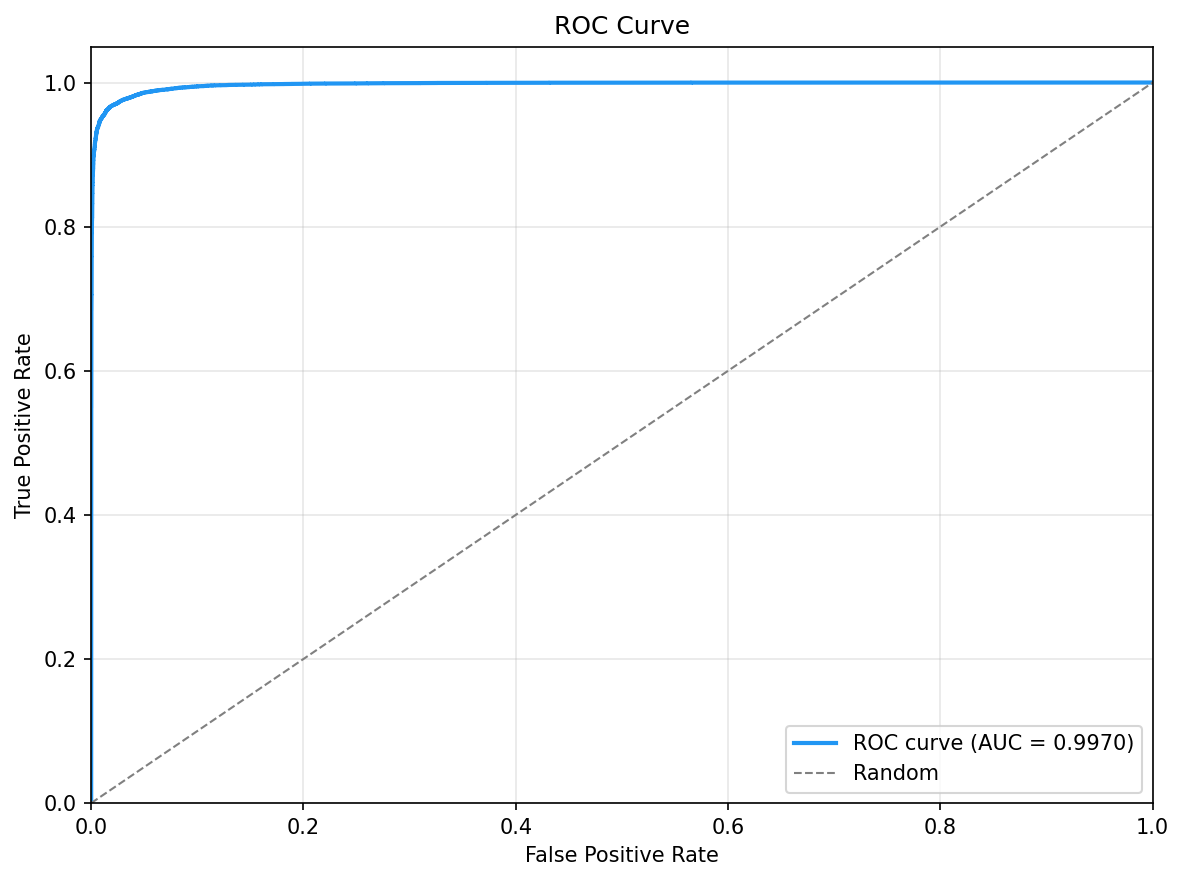
\includegraphics[width=\linewidth]{../../artifacts/results/roc_curve.png}
    \caption{Đường cong ROC (AUC = 0,9970)}
    \label{fig:roc}
  \end{subfigure}
  \caption{Kết quả đánh giá trên tập kiểm tra}
  \label{fig:eval_results}
\end{figure}

\begin{figure}[H]
  \centering
  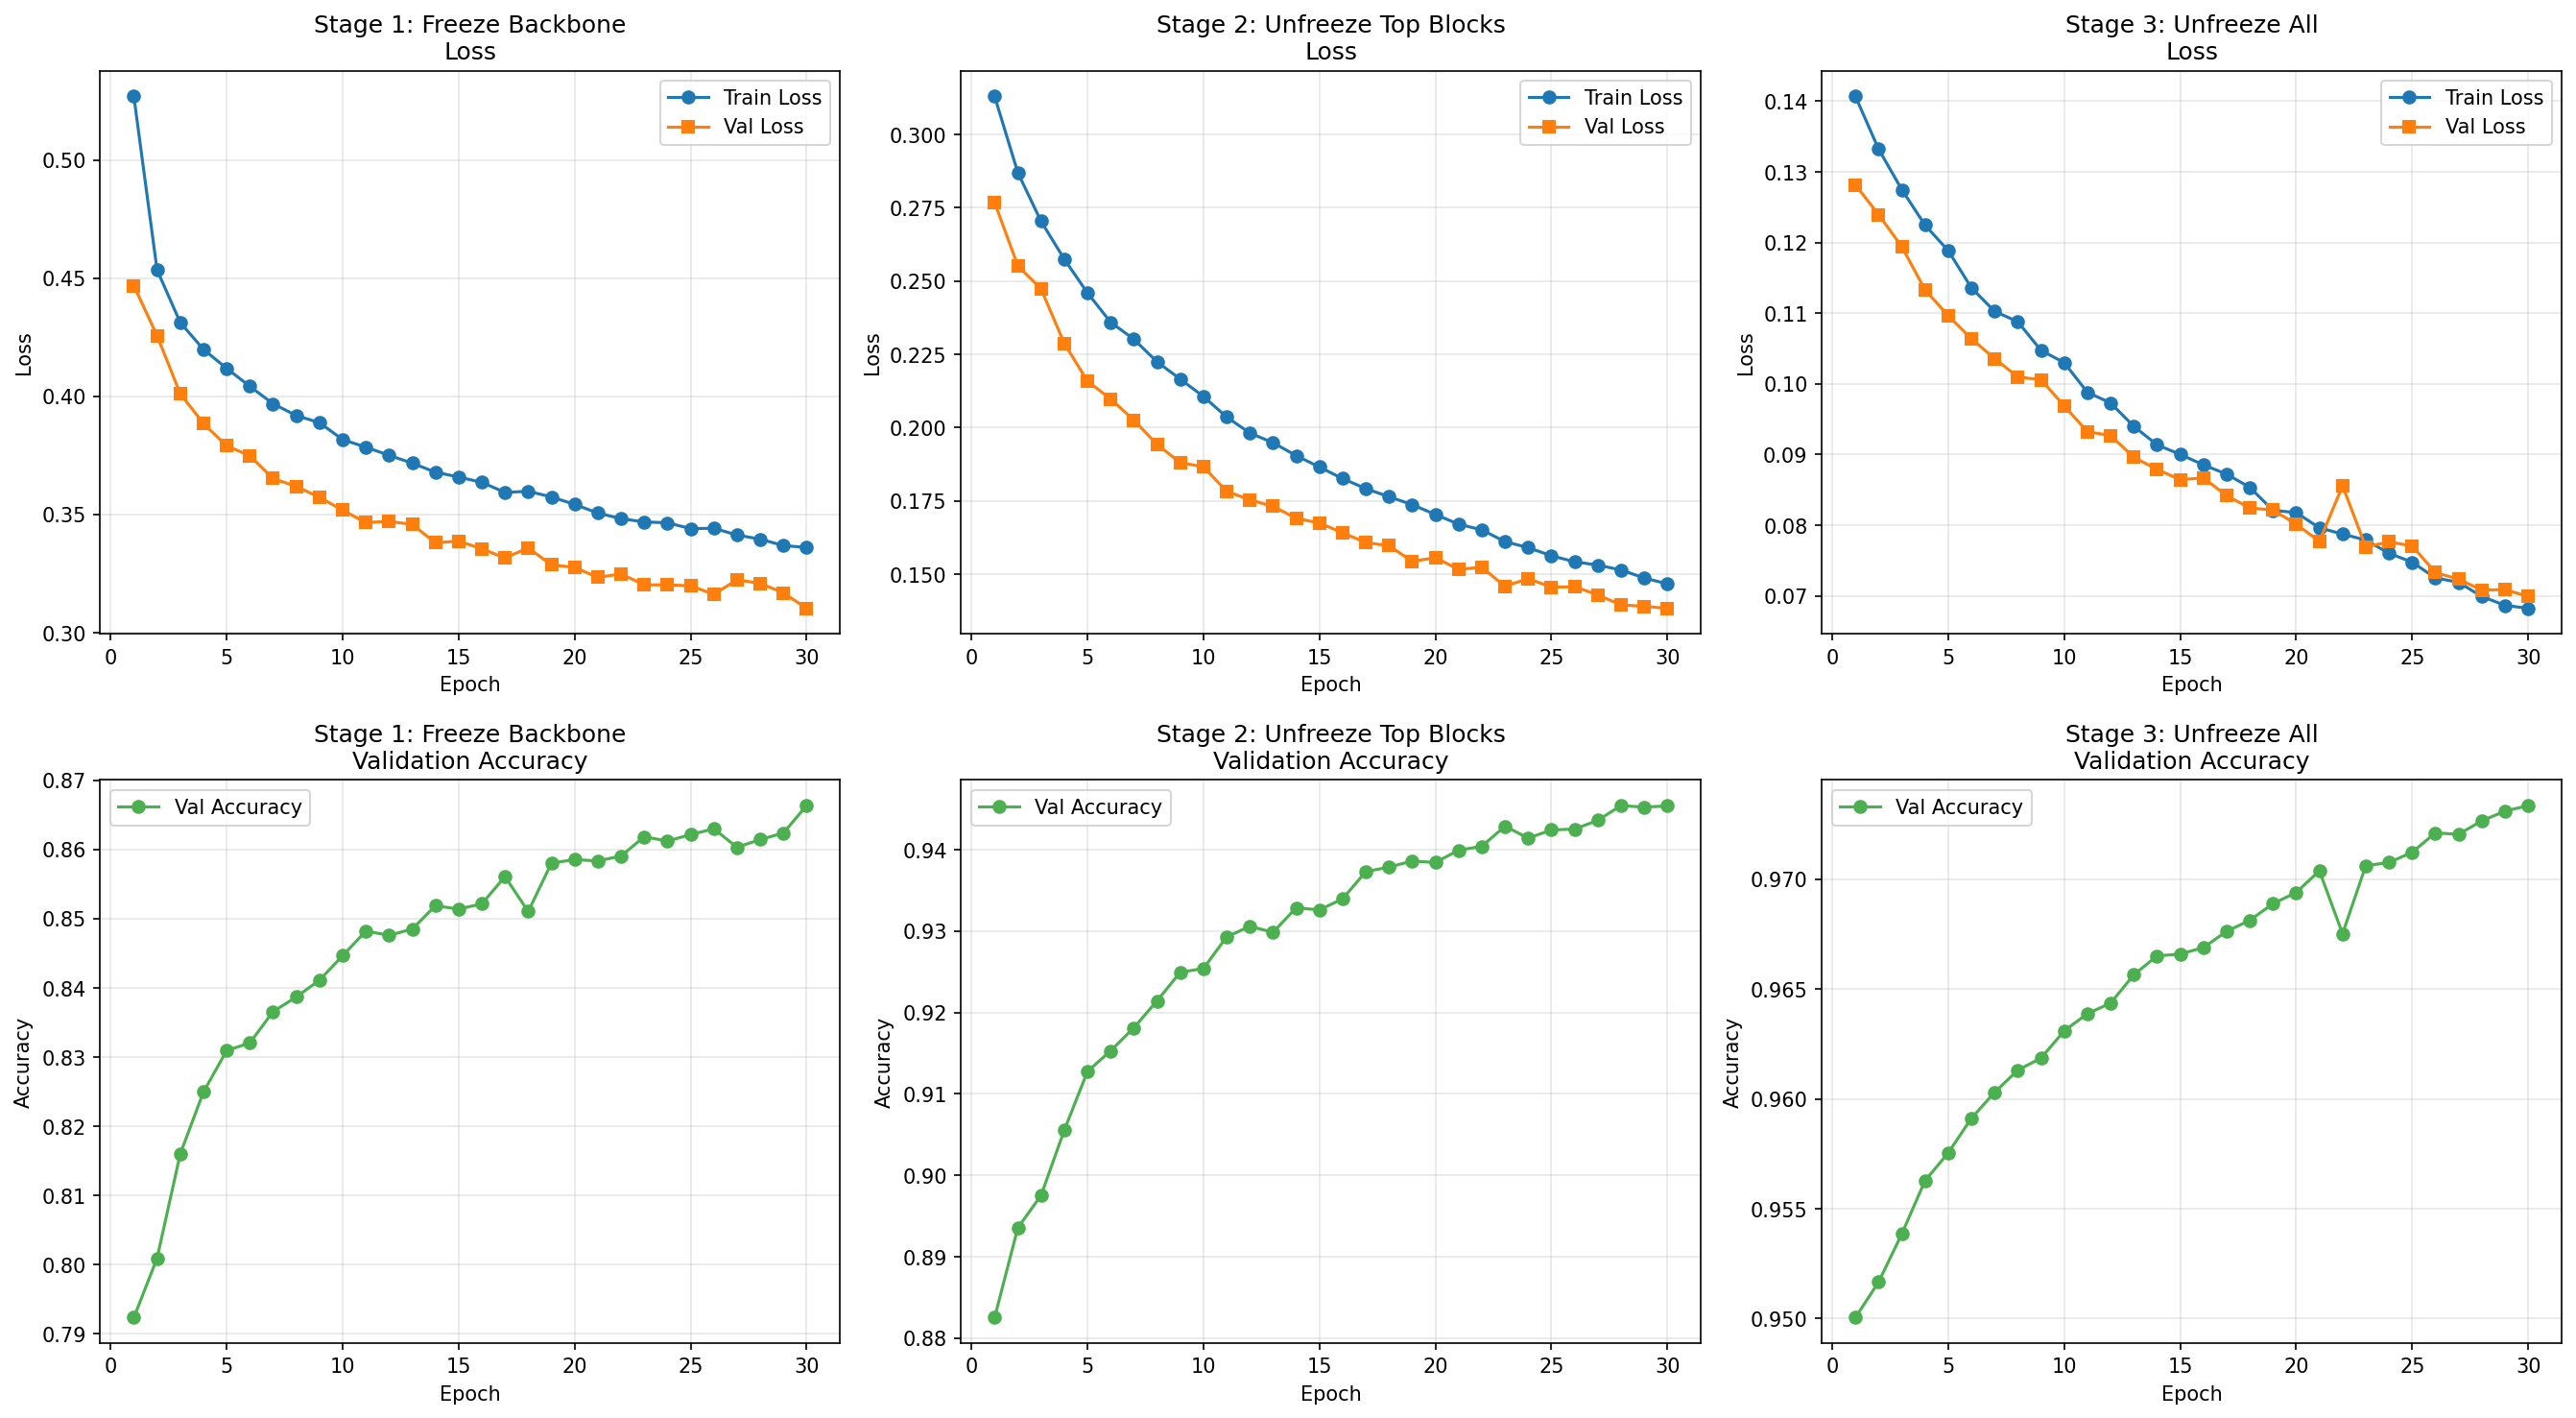
\includegraphics[width=0.9\linewidth]{../../artifacts/results/training_curves.png}
  \caption{Đường cong val\_loss và val\_accuracy theo epoch của 3 giai đoạn huấn luyện}
  \label{fig:training_curves}
\end{figure}

\subsection{Đánh Giá Cross-Generator}

Bài kiểm tra cross-generator thực hiện theo quy trình hold-out: lần lượt giữ lại từng bộ dữ liệu làm tập kiểm tra, huấn luyện mô hình trên ba bộ còn lại, sau đó đánh giá trên bộ bị giữ lại. Quy trình này được lặp lại bốn lần --- một lần cho mỗi bộ dữ liệu. Hình~\ref{fig:cross_gen_scheme} minh họa sơ đồ tổng quát của quy trình này.

\begin{figure}[H]
  \centering
  \begin{tikzpicture}[
    every node/.style={font=\footnotesize},
    trn/.style   = {rectangle, draw=uitblue, fill=uitblue!10, rounded corners=3pt,
                    minimum width=5.0cm, minimum height=0.75cm, align=center},
    hld/.style   = {rectangle, draw=red!60, fill=red!8, rounded corners=3pt,
                    minimum width=1.9cm, minimum height=0.75cm, align=center},
    res/.style   = {rectangle, draw=green!60!black, fill=green!7, rounded corners=3pt,
                    minimum width=2.2cm, minimum height=0.75cm, align=center},
    arr/.style   = {-Stealth, semithick}
  ]
    % Column headers
    \node[font=\footnotesize\bfseries] at (-1.2,  0.55) {Holdout};
    \node[font=\footnotesize\bfseries] at ( 3.1,  0.55) {Huấn luyện (3 bộ)};
    \node[font=\footnotesize\bfseries] at ( 7.0,  0.55) {Accuracy};
    \node[font=\footnotesize\bfseries] at ( 9.4,  0.55) {AUC-ROC};

    % Row 1
    \node[hld] (h1) at (-1.2,  0)    {StyleGAN};
    \node[trn] (t1) at ( 3.1,  0)    {Deepfake + HardFake + ciplab};
    \node[res] (a1) at ( 7.0,  0)    {99,04\%};
    \node[res] (u1) at ( 9.4,  0)    {99,95\%};
    \draw[arr] (t1.east) -- (a1.west);

    % Row 2
    \node[hld] (h2) at (-1.2, -1.15) {Deepfake};
    \node[trn] (t2) at ( 3.1, -1.15) {StyleGAN + HardFake + ciplab};
    \node[res] (a2) at ( 7.0, -1.15) {96,50\%};
    \node[res] (u2) at ( 9.4, -1.15) {99,55\%};
    \draw[arr] (t2.east) -- (a2.west);

    % Row 3
    \node[hld] (h3) at (-1.2, -2.3)  {HardFake};
    \node[trn] (t3) at ( 3.1, -2.3)  {StyleGAN + Deepfake + ciplab};
    \node[res] (a3) at ( 7.0, -2.3)  {90,77\%};
    \node[res] (u3) at ( 9.4, -2.3)  {97,07\%};
    \draw[arr] (t3.east) -- (a3.west);

    % Row 4 (ciplab — red highlight)
    \node[hld, fill=red!15] (h4) at (-1.2, -3.45) {ciplab};
    \node[trn]              (t4) at ( 3.1, -3.45) {StyleGAN + Deepfake + HardFake};
    \node[res, fill=red!15] (a4) at ( 7.0, -3.45) {53,36\%};
    \node[res, fill=red!15] (u4) at ( 9.4, -3.45) {53,44\%};
    \draw[arr] (t4.east) -- (a4.west);
  \end{tikzpicture}
  \caption{Sơ đồ quy trình đánh giá cross-generator (hold-out từng bộ dữ liệu).
           Ô đỏ đậm: bộ ciplab gây sụp đổ hoàn toàn khi bị giữ lại.}
  \label{fig:cross_gen_scheme}
\end{figure}

\begin{table}[H]
  \centering
  \caption{Kết quả cross-generator evaluation đầy đủ (5 độ đo)}
  \label{tab:cross_gen}
  \begin{tabular}{lrrrrr}
    \toprule
    \textbf{Holdout} & \textbf{Acc} & \textbf{Prec} & \textbf{Recall} & \textbf{F1} & \textbf{AUC} \\
    \midrule
    140k-StyleGAN & 99,04\% & 98,93\% & 99,13\% & 99,03\% & 99,95\% \\
    Deepfake-Real & 96,50\% & 97,11\% & 96,55\% & 96,83\% & 99,55\% \\
    Hard-FakeReal & 90,77\% & 88,46\% & 93,88\% & 91,09\% & 97,07\% \\
    ciplab        & 53,36\% & 50,88\% & 20,71\% & 29,44\% & 53,44\% \\
    \bottomrule
  \end{tabular}
  \newline
  {\small Nguồn: \texttt{reports/cross\_generator/cross\_generator\_metrics.json}}
\end{table}

\subsection{Đánh Giá Robustness}

\begin{table}[H]
  \centering
  \caption{Kết quả robustness evaluation}
  \label{tab:robustness}
  \begin{tabular}{lrrr}
    \toprule
    \textbf{Điều kiện nhiễu} & \textbf{Accuracy} & \textbf{F1-Score} & \textbf{AUC-ROC} \\
    \midrule
    Baseline (không nhiễu) & 0,9733 & 0,9745 & 0,9970 \\
    JPEG nén $q=70$        & 82,33\% & 85,32\% & 95,97\% \\
    JPEG nén $q=50$        & 79,77\% & 83,45\% & 93,30\% \\
    JPEG nén $q=30$        & 78,60\% & 82,48\% & 90,30\% \\
    Downscale 50\%         & 85,39\% & 85,60\% & 93,58\% \\
    Downscale 25\%         & 72,87\% & 75,85\% & 80,40\% \\
    Gaussian blur $\sigma=1$ & 90,45\% & 90,29\% & 97,76\% \\
    Gaussian blur $\sigma=2$ & 73,65\% & 73,84\% & 82,11\% \\
    \bottomrule
  \end{tabular}
  \newline
  {\small Nguồn: \texttt{reports/robustness/robustness\_metrics.json}}
\end{table}

\subsection{Nhận Xét}

\subsubsection{Đánh Giá Tổng Quan}

Mô hình EfficientNet-B0 sau Giai đoạn 3 đạt kết quả xuất sắc trên tập kiểm tra chuẩn với Accuracy 97,33\%, F1-Score 97,45\% và AUC-ROC 99,70\%. Val accuracy cải thiện tổng cộng $+10{,}71$ điểm phần trăm từ Giai đoạn 1 đến Giai đoạn 3, xác nhận hiệu quả của chiến lược progressive unfreezing.

\subsubsection{Đánh Giá Theo Từng Độ Đo}

\textbf{Precision (0,9773):} Khi mô hình dự đoán một ảnh là giả, xác suất đúng đạt 97,73\%. Precision cao bác bỏ giả thuyết mô hình thiên vị về lớp đa số (53\% Fake).

\textbf{Recall (0,9718):} Mô hình phát hiện được 97,18\% tổng số ảnh giả thực tế. Khoảng cách nhỏ giữa Precision và Recall ($0{,}55$ pp) cho thấy mô hình không thiên lệch đáng kể về phía nào.

\textbf{AUC-ROC (0,9970):} Gần hoàn hảo --- mô hình có khả năng phân tách xác suất thật/giả rất tốt ở mọi mức ngưỡng.

\subsubsection{Phân Tích Nguyên Nhân Thành Công}

\begin{itemize}
  \item \textbf{Quy mô dữ liệu đa nguồn:} 316.530 ảnh từ 4 phương pháp sinh buộc mô hình học đặc trưng phổ quát thay vì phụ thuộc vào artifact của một phương pháp cụ thể.
  \item \textbf{Progressive unfreezing:} Ngăn catastrophic forgetting, cho phép backbone thích nghi dần với domain khuôn mặt.
  \item \textbf{Mixed precision FP16:} Cho phép batch size 128, cung cấp gradient estimate ổn định hơn.
  \item \textbf{EarlyStopping không kích hoạt:} Cho thấy 30 epochs là hợp lý --- mô hình chưa overfitting khi kết thúc; tăng thêm epochs có thể cải thiện thêm.
\end{itemize}

\subsubsection{Trực Quan Hóa Grad-CAM}

Grad-CAM được thực hiện trên 32 ảnh mẫu (4 Real + 4 Fake $\times$ 4 nguồn), sử dụng checkpoint Stage~3 với lớp mục tiêu là \texttt{backbone.blocks[-1]} (MBConv block cuối của EfficientNet-B0). Kết quả đạt 30/32 dự đoán đúng (93,8\%) trên tập mẫu này --- hai ảnh sai đều thuộc bộ ciplab, nhất quán với kết quả cross-generator (AUC 53,44\%).

\begin{figure}[H]
  \centering
  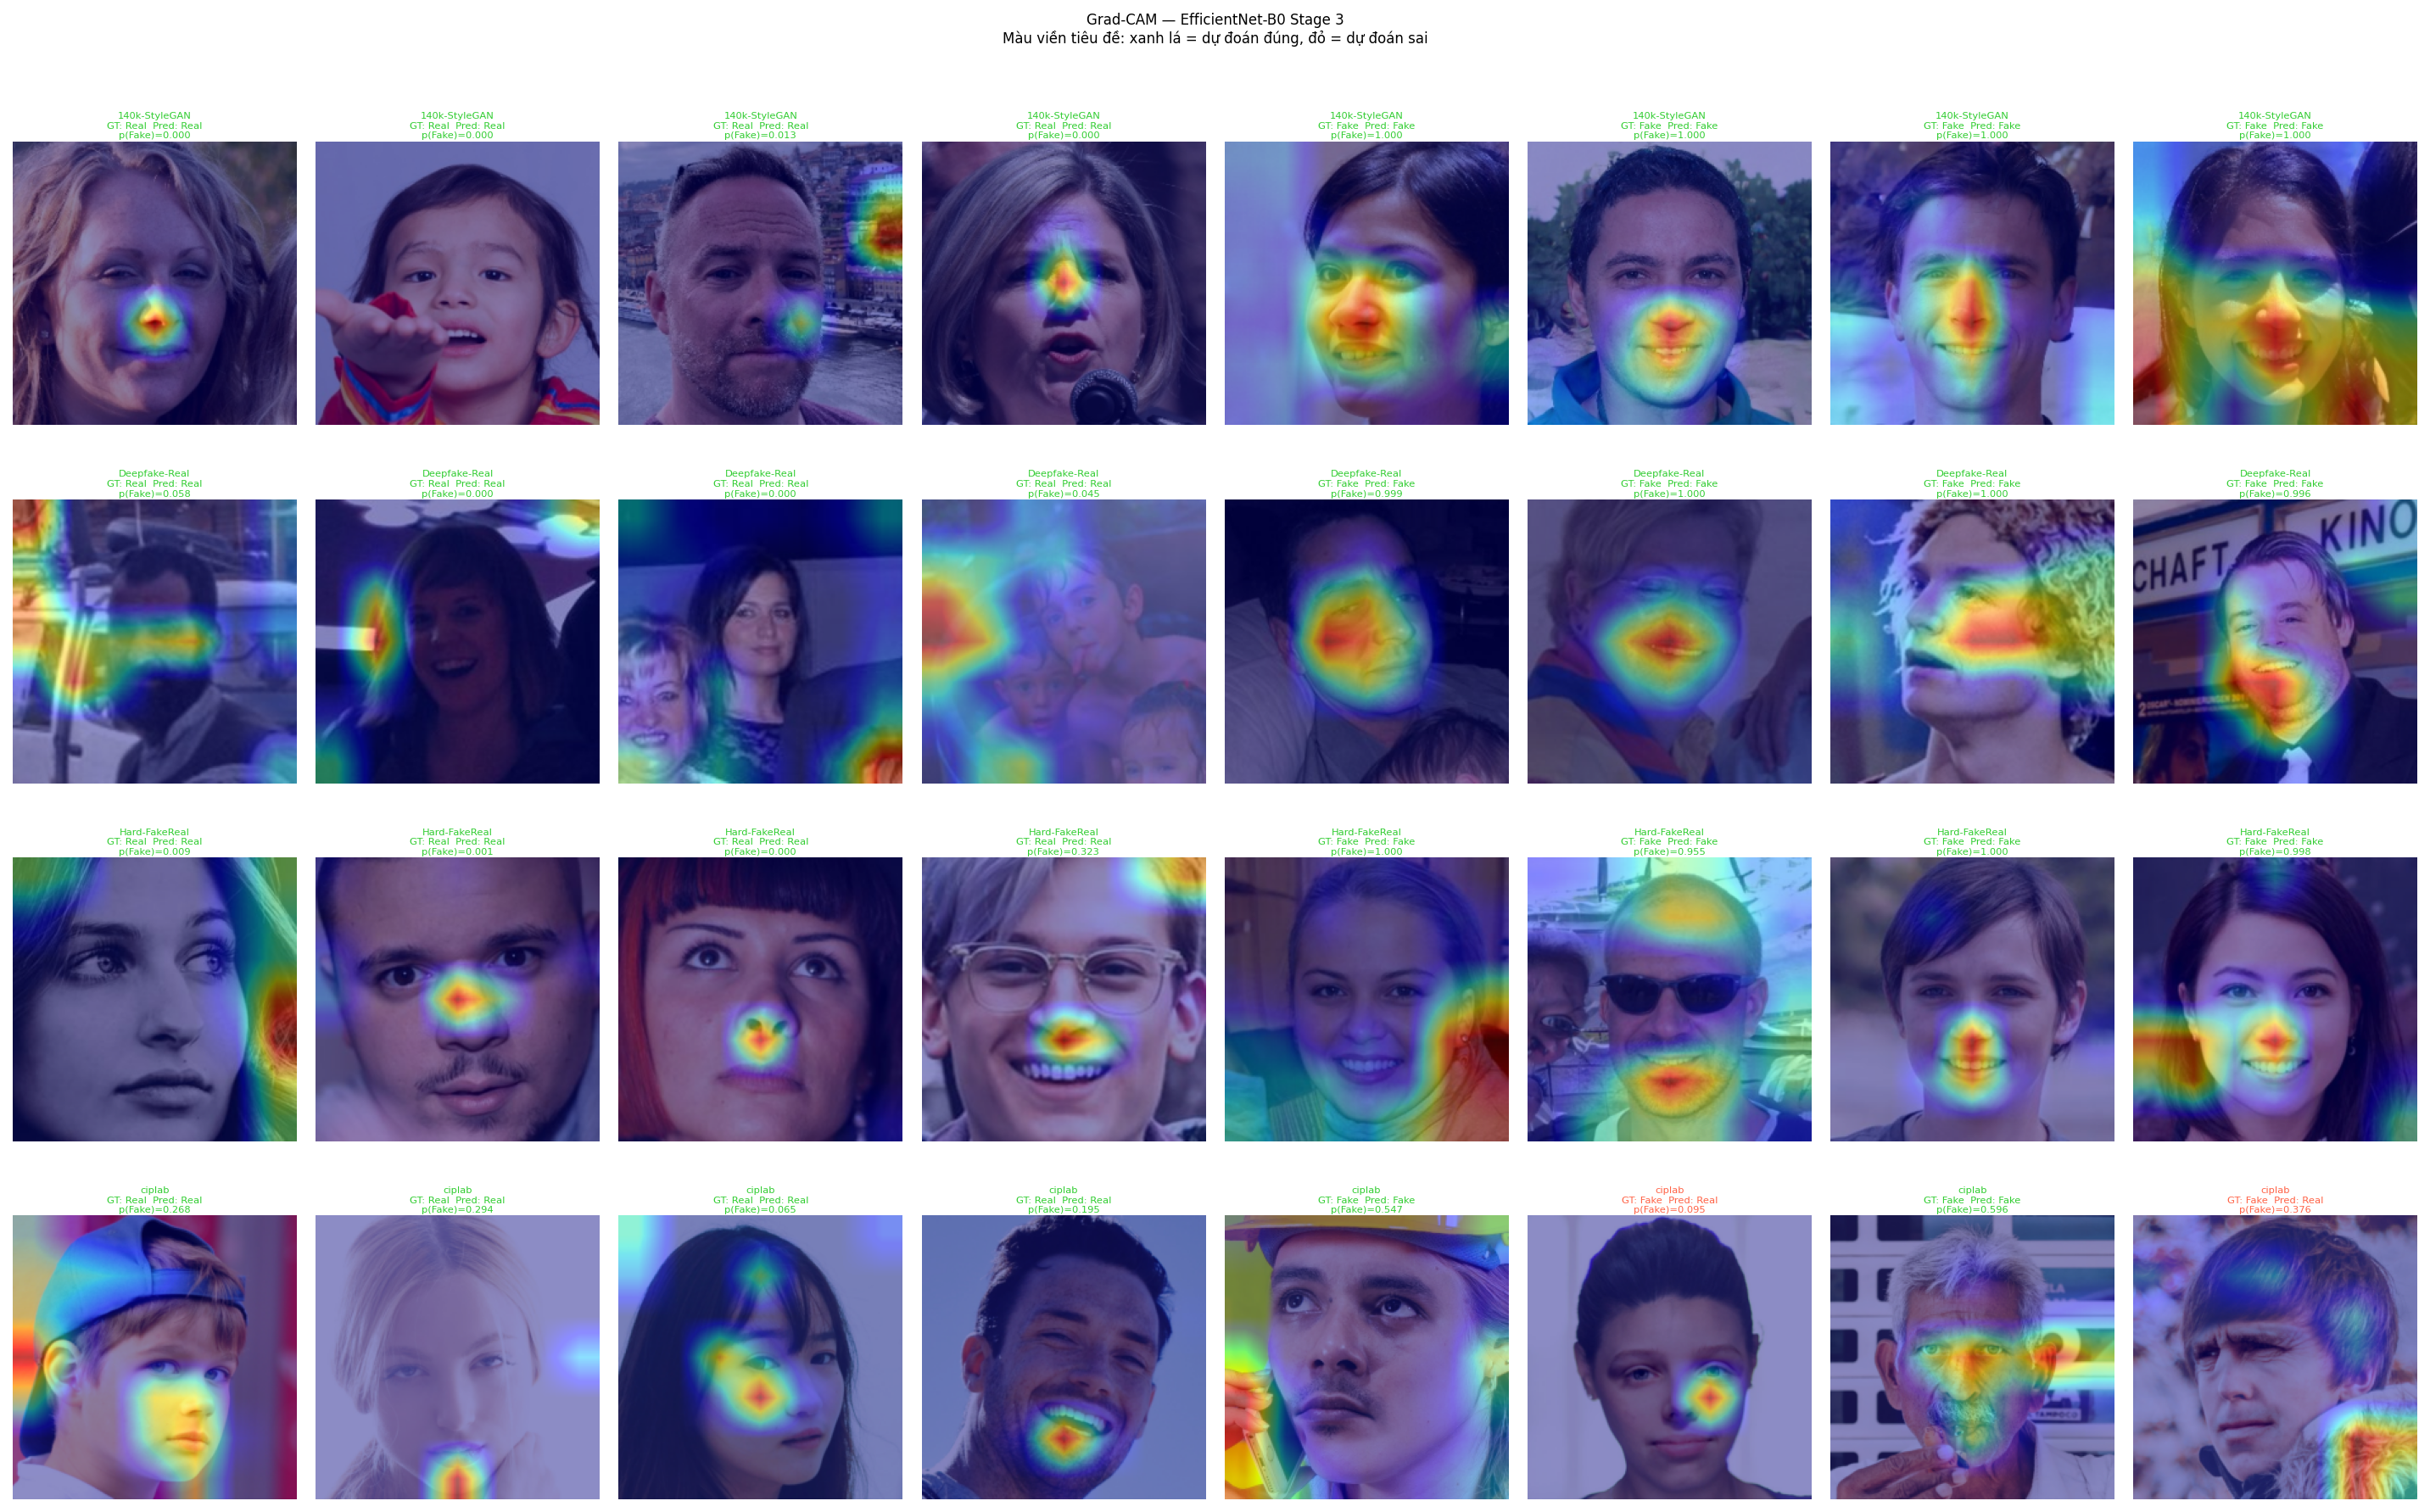
\includegraphics[width=\linewidth]{../gradcam/gradcam_grid.png}
  \caption{Grid Grad-CAM overlay 32 ảnh mẫu (4 nguồn $\times$ 4 Real + 4 Fake). Tiêu đề xanh lá = dự đoán đúng, đỏ = sai.}
  \label{fig:gradcam_grid}
\end{figure}

Quan sát vùng kích hoạt theo nguồn cho thấy:
\begin{itemize}
  \item \textbf{140k-StyleGAN và Hard-FakeReal:} Activation tập trung rõ ràng vào vùng trung tâm khuôn mặt (mắt, sống mũi) và lan sang biên tóc--da --- nơi artifact GAN phổ biến nhất. Cả 8/8 mẫu đúng ở cả hai nguồn.
  \item \textbf{Deepfake-Real:} Activation phân bổ rộng hơn trên toàn khuôn mặt, đặc biệt ở vùng mắt và biên ghép khuôn mặt --- đúng với cơ chế artifact của manipulation-based deepfake. Đạt 8/8.
  \item \textbf{ciplab:} Heatmap kém tập trung, thường lan ra vùng nền hoặc cổ --- cho thấy mô hình không tìm được vùng artifact đặc trưng của nguồn này. Hai ảnh sai có activation phân tán toàn ảnh.
\end{itemize}

Kết quả xác nhận mô hình học chiến lược phát hiện dựa trên vùng khuôn mặt có ngữ nghĩa thay vì đặc trưng màu sắc toàn cục --- tín hiệu tích cực về tính tin cậy. Sự kém tập trung trên ciplab nhất quán với giới hạn cross-generator và chỉ ra rằng artifact ciplab GAN nằm ngoài không gian đặc trưng đã học.

\subsection{Phân Tích Lỗi}

Dựa trên ma trận nhầm lẫn, kết quả cross-generator, kết quả robustness và quan sát Grad-CAM, các trường hợp lỗi phân loại được phân thành ba nhóm chính:

\textbf{Nhóm 1 --- False Negative: ảnh giả bị phân loại là thật.}
Nhóm này chủ yếu gồm ảnh từ bộ ciplab khi holdout (Recall chỉ 20,71\%) và một phần từ Hard-FakeReal. Đặc điểm chung là không có artifact tần số cao rõ ràng --- Grad-CAM cho heatmap phân tán. Đây là trường hợp mô hình thiếu đặc trưng phân biệt thực sự, không thể cải thiện bằng hyperparameter tuning mà cần bổ sung dữ liệu từ chính generator đó.

\textbf{Nhóm 2 --- False Positive: ảnh thật bị phân loại là giả.}
Nhóm này tăng mạnh khi ảnh bị nén JPEG. Tại $q=70$, Precision giảm từ 97,73\% xuống 75,88\%, tức là gần 1/4 ảnh bị cảnh báo nhầm là giả. Nguyên nhân: nén JPEG tạo ra blocking artifact ở tần số trung-cao tương tự artifact GAN, làm mô hình nhầm. Đây là lỗi hệ thống có thể giảm bằng cách thêm \texttt{ImageCompression} vào pipeline augmentation.

\textbf{Nhóm 3 --- Lỗi do mất thông tin nặng.}
Khi downscale $\times 0{,}25$ hoặc Gaussian blur $\sigma=2$, cả False Negative lẫn False Positive đều tăng vì thông tin tần số cao --- nguồn đặc trưng chính của mô hình --- bị xóa vĩnh viễn. Không có biện pháp tiền xử lý nào có thể phục hồi thông tin đã mất; chỉ có super-resolution trước khi phân loại có thể giảm nhẹ tác động.

\begin{table}[H]
  \centering
  \caption{Tóm tắt phân tích lỗi theo điều kiện}
  \label{tab:error_analysis}
  \begin{tabularx}{\linewidth}{lXl}
    \toprule
    \textbf{Điều kiện} & \textbf{Loại lỗi chủ đạo} & \textbf{Biện pháp đề xuất} \\
    \midrule
    ciplab holdout    & FN cao (Recall 20,71\%) & Bổ sung ảnh ciplab vào train \\
    Hard-FakeReal holdout & FN tăng (Acc 90,77\%) & Tăng augmentation độ khó \\
    JPEG $q \leq 70$  & FP tăng (Prec giảm $\approx$22 pp) & Thêm \texttt{ImageCompression} augmentation \\
    Downscale $\times 0{,}25$ & Cả FN và FP tăng & Thêm downscale augmentation \\
    Blur $\sigma=2$   & Cả FN và FP tăng & Thêm Gaussian blur augmentation \\
    \bottomrule
  \end{tabularx}
\end{table}

\section{Ứng Dụng Thực Nghiệm}

\subsection{Pipeline Inference}

\subsection{Sơ Đồ Pipeline Inference}

Hình~\ref{fig:inference_pipeline} trực quan hóa từng bước trong quy trình phân loại một ảnh mới, từ file đầu vào đến quyết định Real/Fake cuối cùng.

\begin{figure}[H]
  \centering
  \begin{tikzpicture}[
    node distance=0.52cm,
    every node/.style={font=\small},
    proc/.style = {rectangle, draw=uitblue, fill=uitblue!8, rounded corners=3pt,
                   minimum width=9.5cm, minimum height=0.88cm, align=center},
    dec/.style  = {diamond, draw=orange!70!black, fill=orange!8, aspect=3,
                   minimum height=1.1cm, align=center},
    res/.style  = {rectangle, draw=green!60!black, fill=green!7, rounded corners=3pt,
                   minimum width=3.5cm, minimum height=0.8cm, align=center},
    arr/.style  = {-Stealth, semithick}
  ]
    \node[proc] (i1) {Ảnh đầu vào (định dạng bất kỳ)};
    \node[proc, below=of i1] (i2) {\texttt{PIL.Image.open()} $\to$ \texttt{convert("RGB")}};
    \node[proc, below=of i2] (i3) {Resize($224\times224$) $\to$ Normalize(ImageNet) $\to$ \texttt{ToTensorV2}};
    \node[proc, below=of i3] (i4) {\texttt{unsqueeze(0)} --- Thêm batch dimension};
    \node[proc, below=of i4] (i5) {\texttt{model.eval()} \quad Forward pass};
    \node[proc, below=of i5] (i6) {\texttt{torch.sigmoid(logit)} $\to$ xác suất $p \in [0,1]$};
    \node[dec,  below=0.65cm of i6] (dec) {$p > 0{,}5$?};
    \node[res, below left=0.65cm and 1.6cm of dec]  (fake) {\textbf{Fake}\\(Ảnh giả mạo)};
    \node[res, below right=0.65cm and 1.6cm of dec] (real) {\textbf{Real}\\(Ảnh thật)};

    \foreach \a/\b in {i1/i2, i2/i3, i3/i4, i4/i5, i5/i6, i6/dec}
      \draw[arr] (\a.south) -- (\b.north);

    \draw[arr] (dec.south west)
      -- node[left, font=\footnotesize] {Có} (fake.north);
    \draw[arr] (dec.south east)
      -- node[right, font=\footnotesize] {Không} (real.north);
  \end{tikzpicture}
  \caption{Pipeline inference phân loại ảnh mới (ngưỡng mặc định 0,5)}
  \label{fig:inference_pipeline}
\end{figure}

\begin{lstlisting}[style=python, caption={Pipeline phân loại ảnh mới}]
from PIL import Image
import torch, albumentations as A
from albumentations.pytorch import ToTensorV2

transform = A.Compose([
    A.Resize(224, 224),
    A.Normalize(mean=[0.485,0.456,0.406],
                std=[0.229,0.224,0.225]),
    ToTensorV2()
])

model.eval()
with torch.no_grad():
    img = transform(image=np.array(Image.open(path).convert("RGB")))
    logit = model(img["image"].unsqueeze(0).to(device))
    prob  = torch.sigmoid(logit).item()
    label = "Fake" if prob > 0.5 else "Real"
\end{lstlisting}

Ngưỡng mặc định là $0{,}5$. Trong ứng dụng ưu tiên Recall cao (không bỏ sót ảnh giả), ngưỡng có thể được hạ xuống $0{,}3$--$0{,}4$ dựa trên đường ROC.

\chapter{KẾT LUẬN}

\section{Tóm Tắt Đề Tài}

Đề tài nghiên cứu bài toán phân loại nhị phân ảnh khuôn mặt thật và ảnh khuôn mặt do AI tổng hợp --- một vấn đề kỹ thuật có ý nghĩa xã hội cấp thiết trong bối cảnh các công cụ sinh ảnh bằng GAN và diffusion models ngày càng tạo ra nội dung photorealistic khó phân biệt bằng mắt thường. Đề tài xây dựng pipeline hoàn chỉnh từ thu thập và hợp nhất bốn bộ dữ liệu Kaggle đa dạng (316.530 ảnh sau dedup) đến huấn luyện mô hình EfficientNet-B0 \cite{tan2019efficientnet} theo chiến lược fine-tuning 3 giai đoạn (progressive unfreezing), đạt Accuracy 97,33\%, F1-Score 97,45\% và AUC-ROC 99,70\% trên tập kiểm tra độc lập. Ngoài đánh giá chuẩn, đề tài thiết kế thêm bài kiểm tra cross-generator để đo khả năng tổng quát hóa, bài kiểm tra robustness để đánh giá độ bền dưới nhiễu thực tế, và trực quan hóa Grad-CAM \cite{selvaraju2017gradcam} để giải thích cơ chế quyết định của mô hình.

\section{Đóng Góp Của Đề Tài}

Đề tài thực hiện năm đóng góp cụ thể:

\begin{enumerate}
  \item \textbf{Pipeline dữ liệu đa nguồn quy mô lớn:} Xây dựng quy trình hợp nhất bốn bộ dữ liệu Kaggle với dedup MD5 và stratified split 70/15/15, tạo tập huấn luyện 221.571 ảnh đa dạng hơn so với các nghiên cứu thường sử dụng một nguồn đơn lẻ.

  \item \textbf{Chiến lược huấn luyện 3 giai đoạn có kiểm soát:} Áp dụng progressive unfreezing (Head-only $\to$ Partial unfreeze blocks 5--6 $\to$ Full fine-tune) kết hợp EarlyStopping và ReduceLROnPlateau, với siêu tham số quản lý tập trung qua \texttt{train\_config.yaml}. Val accuracy cải thiện rõ rệt: 86,63\% $\to$ 94,54\% $\to$ 97,34\%.

  \item \textbf{Đánh giá cross-generator có hệ thống:} Thực hiện hold-out evaluation theo từng bộ dữ liệu nguồn để định lượng khả năng tổng quát hóa thực tế --- quan trọng hơn benchmark in-distribution thông thường.

  \item \textbf{Đánh giá robustness với nhiễu thực tế:} Kiểm tra JPEG compression ($q = 70/50/30$), downscale (50\%/25\%) và Gaussian blur ($\sigma = 1/2$), phản ánh điều kiện ảnh phổ biến khi chia sẻ qua mạng xã hội.

  \item \textbf{Explainability qua Grad-CAM:} Cung cấp bằng chứng trực quan về vùng ảnh mô hình tập trung khi phân loại, tăng tính minh bạch và hỗ trợ tin cậy hóa hệ thống AI trong ứng dụng thực tế.
\end{enumerate}

\chapter{HƯỚNG PHÁT TRIỂN ĐỀ TÀI}

Dựa trên kết quả thực nghiệm và các giới hạn được xác định, sáu hướng phát triển được đề xuất kèm phân tích kỹ thuật và mức độ ưu tiên.

\section{Mở Rộng Sang Ảnh Từ Diffusion Models Thế Hệ Mới}

\textbf{Ưu tiên: Cao nhất.} Tập dữ liệu hiện tại chủ yếu bao gồm ảnh GAN (StyleGAN2, manipulation-based). Các mô hình khuếch tán (Stable Diffusion, Midjourney, DALL-E~3) tạo ra artifact hoàn toàn khác về cấu trúc tần số --- quá trình sinh ảnh theo từng bước khử nhiễu tạo ra phân bố năng lượng tần số khác biệt so với quá trình sinh GAN một bước. Mở rộng tập huấn luyện với ảnh từ các generator này --- theo hướng của GenImage~\cite{zhu2023genimage} và AI-Face~\cite{lin2025aiface} --- là bước cần thiết để duy trì hiệu suất thực tế trước làn sóng công cụ sinh ảnh mới.

\textbf{Gợi ý triển khai:} Thu thập thêm ít nhất 50.000 ảnh từ Stable Diffusion v2/SDXL và Midjourney v6 qua các bộ dữ liệu công khai (ArtiFact, GenImage~\cite{zhu2023genimage}). Huấn luyện lại từ Giai đoạn~2 (partial unfreeze) với tập dữ liệu mở rộng, thay vì từ đầu, để tận dụng đặc trưng đã học từ GAN.

\section{Thử Nghiệm Kiến Trúc Backbone Mạnh Hơn}

EfficientNet-B0 đạt kết quả tốt nhờ cân bằng giữa tốc độ và độ chính xác. Các kiến trúc backbone tiềm năng cho nghiên cứu tiếp theo được trình bày trong Bảng~\ref{tab:future_backbones}.

\begin{table}[H]
  \centering
  \caption{Các kiến trúc backbone tiềm năng cho nghiên cứu tiếp theo}
  \label{tab:future_backbones}
  \begin{tabularx}{\linewidth}{lXrl}
    \toprule
    \textbf{Kiến trúc} & \textbf{Ưu điểm chính} & \textbf{Tham số} & \textbf{Độ phức tạp} \\
    \midrule
    EfficientNet-B4 & Cùng họ với B0, dễ thay thế; độ chính xác cao hơn đáng kể & $\approx$19M & Thấp \\
    ConvNeXt-T & Kiến trúc CNN hiện đại, thiết kế lại theo cảm hứng ViT & $\approx$28M & Thấp \\
    ViT-B/16 & Attention toàn cục; bắt được artifact phân tán không gian & $\approx$86M & Trung bình \\
    CLIP-ViT-B/32 & Pretrained trên 400M cặp ảnh--văn bản; đặc trưng ngữ nghĩa phong phú & $\approx$151M & Cao \\
    \bottomrule
  \end{tabularx}
\end{table}

ViT-B/16 đặc biệt thú vị vì cơ chế self-attention toàn cục có thể phát hiện artifact không cục bộ --- loại artifact mà CNN với receptive field giới hạn có thể bỏ qua. Tuy nhiên, ViT yêu cầu lượng dữ liệu lớn hơn để tránh overfitting và thời gian fine-tuning dài hơn.

\section{Phát Hiện Deepfake Trong Video}

Pipeline hiện tại xử lý ảnh tĩnh đơn lẻ. Mở rộng sang video đòi hỏi mô hình hóa tính nhất quán thời gian (temporal consistency): khuôn mặt deepfake trong video thường có nhấp nháy (flickering) hoặc không nhất quán giữa các frame liên tiếp về màu sắc, ánh sáng hoặc hướng nhìn. Kiến trúc tiếp cận tự nhiên là kết hợp CNN (trích xuất đặc trưng từng frame) với LSTM hoặc Transformer (mô hình hóa chuỗi frame).

\textbf{Gợi ý triển khai cụ thể:} Sử dụng EfficientNet-B0 đã fine-tuned (Stage~3) làm feature extractor đóng băng, thêm một Transformer encoder 2--4 lớp trên chuỗi feature vector từ các frame liên tiếp (cửa sổ trượt 16--32 frame). Cách này tận dụng checkpoint đã có mà không cần huấn luyện lại backbone.

\section{Tối Ưu Hóa Cho Triển Khai Thực Tế}

Mô hình Stage~3 hiện có kích thước 52,5~MB và yêu cầu GPU để đạt tốc độ xử lý thời gian thực. Các kỹ thuật nén mô hình được đề xuất theo thứ tự độ phức tạp tăng dần:

\begin{enumerate}
  \item \textbf{Post-training quantization INT8:} Chuyển trọng số từ FP32 sang INT8, giảm kích thước $\approx 4\times$ (xuống $\approx 13$~MB) với mức giảm accuracy thường $< 1\%$ trên EfficientNet-B0. Triển khai dễ dàng qua \texttt{torch.quantization}.

  \item \textbf{Knowledge distillation:} Huấn luyện EfficientNet-Lite0 (student, $\approx 4$~MB) học xác suất mềm từ Stage~3 (teacher). EfficientNet-Lite0 được tối ưu cho mobile với inference engine TFLite và CoreML.

  \item \textbf{Structured pruning:} Loại bỏ các kênh đặc trưng ít quan trọng theo gradient-based importance score; giảm FLOPS 30--50\% với mức giảm accuracy $< 2\%$. Kết hợp với fine-tuning sau pruning (iterative pruning) cho kết quả tốt hơn one-shot pruning.
\end{enumerate}

\section{Đánh Giá Robustness Với Adversarial Examples}

Bài kiểm tra robustness hiện tại giới hạn ở nhiễu tự nhiên (JPEG, blur, downscale). Trong kịch bản tấn công có chủ đích, kẻ xấu có thể tạo perturbation tối thiểu $\delta$ ($\|\delta\|_\infty \leq \varepsilon$) để đánh lừa mô hình phân loại ảnh giả thành thật. Công thức tổng quát:
\begin{equation}
  \mathbf{x}^* = \mathbf{x} + \delta, \quad \|\delta\|_\infty \leq \varepsilon, \quad f(\mathbf{x}^*) \neq f(\mathbf{x})
  \label{eq:adversarial}
\end{equation}

Các phương pháp tấn công chuẩn gồm: FGSM (Fast Gradient Sign Method --- tấn công một bước), PGD (Projected Gradient Descent --- tấn công nhiều bước mạnh hơn) và C\&W (Carlini \& Wagner --- tìm perturbation nhỏ nhất). Adversarial training --- huấn luyện mô hình trên cả ảnh gốc lẫn ảnh adversarial theo phân phối min-max --- là biện pháp phòng thủ hiệu quả nhất hiện tại, mặc dù có thể làm giảm nhẹ accuracy trên ảnh sạch (tradeoff clean-accuracy vs.\ robust-accuracy).

\section{Tích Hợp Cơ Chế Xác Thực Nguồn Gốc Ảnh (C2PA)}

Hướng tiếp cận phát hiện dựa trên đặc trưng thị giác (như đề tài này) luôn là cuộc chạy đua vũ trang với các generator ngày càng tốt hơn. Kết hợp với chuẩn C2PA (Coalition for Content Provenance and Authenticity) tạo ra cơ chế phòng thủ hai lớp bổ sung cho nhau:

\begin{itemize}
  \item \textbf{Lớp 1 --- C2PA metadata:} Camera và phần mềm chỉnh sửa được chứng nhận gắn chữ ký số vào metadata ảnh tại thời điểm chụp/tạo. Metadata này có thể xác minh nguồn gốc mà không cần phân tích nội dung.
  \item \textbf{Lớp 2 --- Phân tích đặc trưng thị giác:} Mô hình học sâu (như đề tài này) phân tích artifact trong nội dung ảnh, không phụ thuộc vào metadata.
\end{itemize}

Hai lớp bổ sung cho nhau vì metadata có thể bị giả mạo hoặc xóa (C2PA không chống được mọi tấn công), trong khi phân tích thị giác có thể bị đánh lừa bởi generator mới. Hệ thống kết hợp hai lớp --- chỉ tin tưởng ảnh khi \textit{cả hai} lớp xác nhận --- cung cấp bảo vệ bền vững hơn bất kỳ lớp đơn lẻ nào.


% ==================== TÀI LIỆU THAM KHẢO ====================
\addcontentsline{toc}{chapter}{Tài Liệu Tham Khảo}
\bibliography{references}

\end{document}
